
\chapter{Introduction}

\clearpage
    
\section[Reflections on the different ...]{Reflections on the different degrees of enjoyment presented to us by the aspect of nature and the study of her laws.}

%In attempting, after a long absence from my native country, to develop the physical phenomena of the globe, and thesimultaneous action of the forces that pervade the regions ofspace, I experience a twofold cause of anxiety. The subject before me is so inexhaustible and so varied, that I fear eitherto fall into the superficiality of the encyclopedist, or to wearythe mind of my reader by aphorisms consisting of mere generalities clothed in dry and dogmatical forms. Undue conciseness often checks the flow of expression, while diffuseness isalike detrimental to a clear and precise exposition of our ideas.Nature is a free domain, and the profound conceptions andenjoyments she awakens within us can only be vividly deine.ated by thought clothed in exalted forms of speech, worthy ofbearing witness to the majesty and greatness of the creation.

\lettrine[lines=4]{\goudy I}{n} attempting, after a long absence from my native country, to develop the physical phenomena of the globe, and the simultaneous action of the forces that pervade the regions of space, I experience a twofold cause of anxiety. The subject before me is so inexhaustible and so varied, that I fear either to fall into the superficiality of the encyclopedist, or to weary the mind of my reader by aphorisms consisting of mere generalities clothed in dry and dogmatical forms. Undue conciseness often checks the flow of expression, while diffuseness is alike detrimental to a clear and precise exposition of our ideas. Nature is a free domain, and the profound conceptions and enjoyments she awakens within us can only be vividly delineated by thought clothed in exalted forms of speech, worthy of bearing witness to the majesty and greatness of the creation.

In considering the study of physical phenomena, not merely in its bearings on the material wants of life, but in its general influence on the intellectual advancement of mankind, we find its noblest and most important result to be a knowledge of the chain of connection, by which all natural forces are linked together, and made mutually dependent upon each other; and it is the perception of these relations that exalts our views and ennobles our enjoyments. Such a result can, however, only be reaped as the fruit of observation and intellect, combined with the spirit of the age, in which are reflected all the varied phases of thought. He who can trace through bygone times, the stream of our knowledge to its primitive source, will learn from history how, for thousands of years, man has labored, amid the ever recurring changes of form, to recognize the invariability of natural laws, and has thus, by the force of mind, gradually subdued a great portion of the physical world to his dominion. In interrogating the history of the past, we trace the mysterious course of ideas yielding the first glimmering perception of the same image of a Cosmos, or harmoniously ordered whole, which, dimly shadowed forth to the human mind in the primitive ages of the world, is now fully revealed to the maturer intellect of mankind as the result of long and laborious observation.

Each of these epochs of the contemplation of the external world -- the earliest dawn of thought and the advanced stage of civilization -- has its own source of enjoyment. In the former, this enjoyment, in accordance with the simplicity of the primitive ages, flowed from an intuitive feeling of the order that was proclaimed by the invariable and successive reappearance of the heavenly bodies, and by the progressive development of organized beings; while in the latter, this sense of enjoyment springs from a definite knowledge of the phenomena of nature. When man began to interrogate nature, and not content with observing, learned to evoke phenomena under definite conditions; when once he sought to collect and record facts, in order that the fruit of his labors might aid investigation after his own brief existence had passed away, the philosophy of Nature cast aside the vague and poetic garb in which she had been enveloped from her origin, and, having assumed a severer aspect, she now weighs the value of observations and substitutes induction and reasoning for conjecture and assumption. The dogmas of former ages survive now only in the superstitions of the people and the prejudices of the ignorant, or are perpetuated in a few systems which, conscious of their weakness, shroud themselves in a veil of mystery. We may also trace the same primitive intuitions in languages exuberant in figurative expressions; and a few of the best chosen symbols engendered by the happy inspiration of the earliest ages, having by degrees lost their vagueness through a better mode of interpretation, are still preserved among our scientific terms.

Nature considered rationally, that is to say, submitted to the process of thought, is a unity in diversity of phenomena; a harmony, blending together all created things; however dissimilar in form and attributes; one great whole (76 7v) animated by the breath of life. The most important result of a rational inquiry into nature is, therefore, to establish the unity and harmony of this stupendous mass of force and matter, to determine with impartial justice what is due to the discoveries of the past and to those of the present, and to analyze the individual parts of natural phenomena without succumbing beneath the weight of the whole. Thus, and thus alone, is it permitted to man, while mindful of the high destiny of his race, to comprehend nature, to lift the veil that shrouds her phenomena, and, as it were, submit the results of observation to the test of reason and of intellect.

In reflecting upon the different degrees of enjoyment presented to us in the contemplation of nature, we find that the first place must be assigned to a sensation, which is wholly independent of an intimate acquaintance with the physical phenomena presented to our view, or of the peculiar character of the region surrounding us. In the uniform plain bounded only by a distant horizon, where the lowly heather, the cistus, or waving grasses, deck the soil; on the ocean shore, where the waves, softly rippling over the beach, leave a track, green with the weeds of the sea; everywhere, the mind is penetrated by the same sense of the grandeur and vast expanse of nature, revealing to the soul, by a mysterious inspiration, the existence of laws that regulate the forces of the universe. Mere communion with nature, mere contact with the free air, exercise a soothing yet strengthening influence on the wearied spirit, calm the storm of passion, and soften the heart when shaken by sorrow to its inmost depths. Everywhere, in every region of the globe, in every stage of intellectual culture, the same sources of enjoyment are alike vouchsafed to man. The earnest and solemn thoughts awakened by a communion with nature intuitively arise from a presentiment of the order and harmony pervading the whole universe, and from the contrast we draw between the narrow limits of our own existence and the image of infinity revealed on every side, whether we look upward to the starry vault of heaven, scan the far-stretching plain before us, or seek to trace the dim horizon across the vast expanse of ocean.

\begin{figure}[h]
    
\includegraphics[width=1\textwidth]{../../pictures/Humboldt&Bonpland_Orenoque}
    \caption{\small Alexander von Humboldt \& Aim\'e Bonpland, Orinocco -- Woodcut (1870) of Otto
       Roth from a drawing by H. Lademann. Image in the public domain.}
 \end{figure}

The contemplation of the individual characteristics of the landscape, and of the conformation of the land in any definite region of the earth, gives rise to a different source of enjoyment, awakening impressions that are more vivid, better defined, and more congenial to certain phases of the mind, than those of which we have already spoken. At one time the heart is stirred by a sense of the grandeur of the face of nature, by the strife of the elements, or, as in Northern Asia, by the aspect of the dreary barrenness of the far-stretching steppes; at another time, softer emotions are excited by the contemplation of rich harvests wrested by the hand of man from the wild fertility of nature, or by the sight of human habitations raised beside some wild and foaming torrent. Here I regard less the degree of intensity than the difference existing in the various sensations that derive their charm and permanence from the peculiar character of the scene.

If I might be allowed to abandon myself to the recollections of my own distant travels, I would instance, among the most striking scenes of nature, the calm sublimity of a tropical night, when the stars, not sparkling, as in our northern skies, shed their soft and planetary light over the gently heaving ocean; or I would recall the deep valleys of the Cordilleras, where the tall and slender palms pierce the leafy veil around them, and waving on high their feathery and arrowlike branches, form, as it were, a ``forest above a forest''\footnote{This expression is taken from a beautiful description of tropical forest scenery in \emph{Paul and Virginia}, by Bernardin de Saint Pierre.}; or I would describe the summit of the Peak of Teneriffe, when a horizontal layer of clouds, dazzling in whiteness, has separated the cone of cinders from the plain below, and suddenly the ascending current pierces the cloudy veil, so that the eye of the traveler may range from the brink of the crater, along the vineclad slopes of Orotava, to the orange gardens and banana groves that skirt the shore. In scenes like these, it is not the peaceful charm uniformly spread over the face of nature that moves the heart, but rather the peculiar physiognomy and conformation of the land, the features of the landscape, the ever-varying outline of the clouds, and their blending with the horizon of the sea, whether it lies spread before us like a smooth and shining mirror, or is dimly seen through the morning mist. All that the senses can but imperfectly comprehend, all that is most awful in such romantic scenes of nature, may become a source of enjoyment to man, by opening a wide field to the creative powers of his imagination. Impressions change with the varying movements of the mind, and we are led by a happy illusion to believe that we receive from the external world that with which we have ourselves invested it.

When far from our native country, after a long voyage, we read for the first time the soil of a tropical land, we experience a certain feeling of surprise and gratification in recognizing, in the rocks that surround us, the same inclined schistose strata, and the same columnar basalt covered with cellular amygdaloids, that we had left in Europe, and whose identity of character, in latitudes so widely different, reminds us that the solidification of the earth's crust is altogether independent of climatic influences. But these rocky masses of schist and of basalt are covered with vegetation of a character with which we are unacquainted, and of a physiognomy wholly unknown to us; and it is then, amid the colossal and majestic forms of an exotic flora, that we feel how wonderfully the flexibility of our nature fits us to receive new impressions, linked together by a certain secret analogy. We so readily perceive the affinity existing among all the forms of organic life, that although the sight of a vegetation similar to that of our native country might at first be most welcome to the eye, as the sweet familiar sounds of our mother tongue are to the ear, we nevertheless, by degrees, and almost imperceptibly, become familiarized with a new home and a new climate. As a true citizen of the world, man everywhere habituates himself to that which surrounds him; yet fearful, as it were, of breaking the links of association that bind him to the home of his childhood, the colonist applies to some few plants in a far distant clime the names he had been familiar with in his native land; and by the mysterious relations existing among all types of organization, the forms of exotic vegetation present themselves to his mind as nobler and more perfect developments of those he had loved in earlier days. Thus do the spontaneous impressions of the untutored mind lead, like the laborious deductions of cultivated intellect, to the same intimate persuasion, that one sole and indissoluble chain binds together all nature.

It may seem a rash attempt to endeavor to separate, into its different elements, the magic power exercised upon our minds by the physical world, since the character of the landscape, and of every imposing scene in nature, depends so materially upon the mutual relation of the ideas and sentiments simultaneously excited in the mind of the observer.

The powerful effect exercised by nature springs, as it were, from the connection and unity of the impressions and emotions produced; and we can only trace their different sources by analyzing the individuality of objects and the diversity of forces.

The richest and most varied elements for pursuing an analysis of this nature present themselves to the eyes of the traveler in the scenery of Southern Asia, in the Great Indian Archipelago, and more especially, too, in the New Continent, where the summits of the lofty Cordilleras penetrate the confines of the aerial ocean surrounding our globe, and where the same subterranean forces that once raised these mountain chains still shake them to their foundation and threaten their downfall.

Graphic delineations of nature, arranged according to systematic views, are not only suited to please the imagination, but may also, when properly considered, indicate the grades of the impressions of which I have spoken, from the uniformity of the seashore, or the barren steppes of Siberia, to the inexhaustible fertility of the torrid zone. If we were even to picture to ourselves Mount Pilatus placed on the Schreckhorn
\footnote{These comparisons are only approximative. The several elevations above the level of the sea are, in accurate numbers, as follows: The Schneekoppe or Riesenkoppe, in Silesia, about 5270 feet, according to Hallaschka. The Righi, 5902 feet, taking the height of the Lake of Lucerne at 1426 feet, according to Eschman. Mount Athos, 6775 feet, according to Captain Gaultier; Mount Pilatus, 7546 feet; Mount \AE tna, 10,871 feet, according to Captain Smyth; or 10,874 feet, according to the barometrical measurement made by Sir John Herschel, and communicated to me in writing in 1825, and 10,899 feet, according to angles of altitude taken by Cacciatore at Palermo (calculated by assuming the terrestrial refraction to be 0.076); the Schreckhorn, 12,383 feet; the Jungfrau, 13,720 feet, according to Tralles; Mont Blanc, 15,775 feet, according to the different measurements considered by Roger (Bibl. Univ., May, 1828, p. 2453), 15,733 feet, according to the measurements taken from Mount Columbier by Carlini in 1821, and 15,748 feet, as measured by the Austrian engineers from Trelod and the Glacier d'Ambin.

The Schneekoppe or Riesenkoppe, in Silesia, about 5270 feet, according to Hallaschka. The Righi, 5902 feet, taking the height of the Lake of Lucerne at 1426 feet, according to Eschman. (See Compte Rendu des Mesures Trigonom\'{e}triques en Suisse, 1840, p. 230.) Mount Athos, 6775 feet, according to Captain Gaultier; Mount Pilatus, 7546 feet; Mount \AE tna, 10,871 feet, according to Captain Smyth; or 10,874 feet, according to the barometrical measurement made by Sir John Herschel, and communicated to me in writing in 1825, and 10,899 feet, according to angles of altitude taken by Cacciatore at Palermo (calculated by assuming the terrestrial refraction to be 0.076); the Schreckhorn, 12,383 feet; the Jungfrau, 13,720 feet, according to Tralles; Mont Blanc, 15,775 feet, according to the different measurements considered by Roger (Bibl. Univ., May, 1828, p. 2453), 15,733 feet, according to the measurements taken from Mount Columbier by Carlini in 1821, and 15,748 feet, as measured by the Austrian engineers from Trelod and the Glacier d'Ambin. ,

The actual height of the Swiss mountains fluctuates, according to Eschman's observations, as much as 25 English feet, owing to the varying thickness of the stratum of snow that covers the summits. Chimborazo is, according to my trigonometrical measurements, 21,421 feet (see Humboldt, Recueil d'Obs. Astr., tome i., p. 73), and Dhawalagiri, 28,074 feet. As there is a difference of 445 feet between the determinations of Blake and Webb, the elevation assigned to the Dhawalagiri (or white mountain, from the Sanskrit dhawala, white, and gi7i, mountain) can not be received with the same confidence as that of the Jawahir, 25,749 feet, since the latter rests on a complete trigonometrical measurement (see Herbert and Hodgson in the As\'{e}at. Res., vol. xiv., p. 189, and Suppl. to Encycl. Brit., vol. iv., p. 643). I have shown elsewhere (Ann. des Sciences Naturelles, Mars, 1825) that the height of the Dhawalagiri (28,074 feet) depends on several elements that have not been ascertained with certainty, such as azimuths and latitudes (Humboldt, Asie Centrale, t. iii., p. 282). It has been believed, but without foundation, that in the Tartaric chain, north of Thibet, opposite to the chain of Kuenlun, there are several snowy summits, whose elevation is about 30,000 English feet (almost twice that of Mont Blanc), or, at any rate, 29,000 feet (see Captain Alexander Gerard's and John Gerard's Journey to the Boorendo Pass, 1840, vol. i., p. 143 and 311). Chimborazo is spoken of in the text only as one of the highest summits of the chain of the Andes; for in the year 1827, the learned and highly gifted traveler, Pentland, in his memorable expedition to Upper Peru (Bolivia), measured the elevation of two mountains situated to the east of Lake Titicaca, viz., the Sorata, 25,200 feet, and the Illimani, 24,000 feet, both greatly exceeding the height of Chimborazo, which is only 21,421 feet, and being nearly equal in elevation to the Jawahir, which is the highest mountain in the Himalaya that has as yet been accurately measured.

Thus Mont Blanc is 5646 feet below Chimborazo; Chimborazo, 3779 feet below the Sorata; the Sorata, 549 feet below the Jawahir, and probably about 2880 feet below the Dhawalagiri. According to a new measurement of the Illimani, by Pentland, in 1838, the elevation of this mountain is given at 23,868 feet, varying only 133 feet from the measurement taken in 1827. The elevations have been given in this note with minute exactness, as erroneous numbers have been introduced into many maps and tables recently published, owing to incorrect redactions of the measurements.

[In the preceding note, taken from those appended to the Introduction in the French translation, rewritten by Humboldt himself, the measurements are given in meters, but these have been converted into English feet, for the greater convenience of the general reader.] -- Tr.}, or the Schneekoppe of Silesia on Mont Blanc, we should not have attained to the height of that great Colossus of the Andes, the Chimborazo, whose height is twice that of Mount \AE tna; and we must pile the Righi, or Mount Athos, on the summit of the Chimborazo, in order to form a just estimate of the elevation of the Dhawalagiri, the highest point of the Himalaya. But although the mountains of India greatly surpass the Cordilleras of South America by their astonishing elevation (which, after being long contested, has at last been confirmed by accurate measurements), they cannot, from their geographical position, present the same inexhaustible variety of phenomena by which the latter are characterized. The impression produced by the grander aspects of nature does not depend exclusively on height. The chain of the Himalaya is placed far beyond the limits of the torrid zone, and scarcely a solitary palm tree is to be found in the beautiful valleys of Kumaoun and Garhwal\footnote{The absence of palms and tree ferns on the temperate slopes of the Himalaya is shown in Don's Flora Nepalensis, 1825, and in the remarkable series of lithographs of Wallich's Flora Indica, whose catalogue contains the enormous number of 7683 Himalaya species, almost all phanerogamic plants, which have as yet been but imperfectly classified. In Nepal (lat. 26° to 27°) there has hitherto been observed only one species of palm, Chamerops martiana, Wall. (Plante Asiat., lib. iii., p. 5, 211), which is found at the height of 5250 English feet above the level of the sea, in the shady valley of Bunipa. The magnificent tree fern Alsophila brunoniana, Wall. (of which a stem 48 feet long has been in the possession of the British Museum since 1831), does not grow in Nepal, but is found on the mountains of Silhet, to the northwest of Calcutta, in lat. 24° 9'. The Nepal fern, Paranema cyathiodes, Don, formerly known as Spheroptera barbata, Wall. (Plante Asiat., lib. i., p. 42, 48), is indeed nearly related to Cyathea, a species of which we saw in the South American Missions of Caripe, measuring 33 feet in height; this is not, however, properly speaking, a tree.
}. On the southern slope of the ancient Paropamisus, in the latitudes of 28 and 34, nature no longer displays the same abundance of tree ferns and arborescent grasses, heliconias and orchidaceous plants, which in tropical regions are to be found even on the highest plateaux of the mountains. On the slope of the Himalaya, under the shade of the Deodora and the broadleaved oak, peculiar to these Indian Alps, the rocks of granite and of mica schist are covered with vegetable forms almost similar to those which characterize Europe and Northern Asia. The species are not identical, but closely analogous in aspect and physiognomy, as, for instance, the juniper, the alpine birch, the gentian, the marsh parnassia, and the prickly species of Ribes\footnote{Ribes nubicola, R. glaciale, R. grossularia. The species which compose the vegetation of the Himalaya are four pines, notwithstanding the assertion of the ancients regarding Eastern Asia (Strabo, lib. 11, p. 510, Cas.), twenty-five oaks, four birches, two chestnuts, seven maples, twelve willows, fourteen roses, three species of strawberry, seven species of Alpine roses (rhododendra), one of which attains a height of 20 feet, and many other northern genera. Large white apes, having black faces, inhabit the wild chestnut tree of Kashmir, which grows to a height of 100 feet, in lat. 33 (see Carl von Hiigels Kaschmir, 1840, 2d pt. 249). Among the Conifer, we find the Pinus deodwara, or deodara (in Sanscrit, d\'{e}wadaru, the timber of the gods), which is nearly allied to Pinus cedrus. Near the limit of perpetual snow flourish the large and showy flowers of the Gentiana venusta, G. Moorcroftiana, Swertia purpurescens, S. speciosa, Parnassia armata, P. nubicola, Poeonia Emodi, Tulipa stellata; and, besides varieties of European genera peculiar to these Indian mountains, true European species, as Leontodon taraxacum, Prunella vulgaris, Galium aparine, and Thlaspi arvense. The heath mentioned by Saunders, in Turner's Travels, and which had been confounded with Calluna vulgaris, is an Andromeda, a fact of the greatest importance in the geography of Asiatic plants. If I have made use, in this work, of the unphilosophical expressions of European genera, European species, growing wild in Asia, c., it has been in consequence of the old botanical language, which, instead of the idea of a large dissemination, or, rather, of the coexistence of organic productions, has dogmatically substituted the false hypothesis of a migration, which, from predilection for Europe, is further assumed to have been from west to east.}. The chain of the Himalaya is also wanting in the imposing phenomena of volcanoes, which in the Andes and in the Indian Archipelago often reveal to the inhabitants, under the most terrific forms, the existence of the forces pervading the interior of our planet.

Moreover, on the southern declivity of the Himalaya, wherethe ascending current deposits the exhalations rising from avigorous Indian vegetation, the region of perpetual snow begins at an elevation of 11,000 or 12,000 feet above the levelof the sea,\footnote{On the southern declivity of the Himalaya, the limit of perpetual snow is 12,978 feet above the level of the sea; on the northern declivity, or, rather, on the peaks which rise above the Thibet, or Tartarian plateau, this limit is at 16,625 feet from 30 to 32 of latitude, while at the equator, in the Andes of Quito, it is 15,790 feet. Such is the result I have deduced from the combination of numerous data furnished by Webb, Gerard, Herbert, and Moorcroft. (See my two memoirs on the mountains of India, in 1816 and 1820, in the Ann. de Chimie et de Physique, t. iii., p. 303; t. xiv., p. 6, 22, 50.) The greater elevation to which the limit of perpetual snow recedes on the Tartarian declivity is owing to the radiation of heat from the neighboring elevated plains, to the purity of the atmosphere, and to the infrequent formation of snow in an air which is both very cold and very dry. (Humboldt, Asie Centrale, t. iii., p. 281-326.) My opinion on the difference of height of the snowline on the two sides of the Himalaya has the high authority of Colebrooke in its favor. He wrote to me in June, 1824, as follows: "I also find, from the data in my possession, that the elevation of the line of perpetual snow is 13,000 feet. On the southern declivity, and at latitude 31, Webb's measurements give me 13,500 feet, consequently 500 feet more than the height deduced from Captain Hedgson's observations. Gerard's measurements fully confirm your opinion that the line of snow is higher on the northern than on the southern side." It was not until the present year (1840) that we obtained the complete and collected journal of the brothers Gerard, published under the supervision of Mr. Lloyd. (Narrative of a Journey from Cawnpoor to the Boorendo Pass, in the Himalaya, by Captain Alexander Gerard and John Gerard, edited by George Lloyd, vol. i., p. 291, 311, 320, 327, and 341.) Many interesting details regarding some localities may be found in the narrative of A Visit to the Shatool, for the Purpose of determining the Line of Perpetual Snow on the southern face of the Himalaya, in August, 1822. Unfortunately, however, these travelers always confound the elevation at which sporadic snow falls with the maximum of the height that the snowline attains on the Thibetian plateau. Captain Gerard distinguishes between the summits that rise in the middle of the plateau, where he states the elevation of the snowline to be between 18,000 and 19,000 feet, and the northern slopes of the chain of the Himalaya, which border on the defile of the Sutledge, and can radiate but little heat, owing to the deep ravines with which they are intersected. The elevation of the village of Tangno is given at only 1300 feet, while that of the plateau surrounding the lake of Minasa is 17,000 feet. Captain Gerard finds the snowline 500 feet lower on the northern slopes, where the chain of the Himalaya is broken through, than toward the southern declivities facing Hindostan, and he there estimates the line of perpetual snow at 15,000 feet. The most striking differences are presented between the vegetation on the Thibetian plateau and that characteristic of the southern slopes of the Himalaya. On the latter, the cultivation of grain is arrested at 9974 feet, and even there the corn has often to be cut when the blades are still green. The extreme limit of forests of tall oaks and deodars is 11,960 feet; that of dwarf birches, 12,983 feet. On the plains, Captain Gerard found pastures up to the height of 17,000 feet; the cereals will grow at 14,100 feet, or even at 18,540 feet; birches with tall stems at 14,100 feet, and copse or brushwood applicable for fuel is found at an elevation of an of 17,000 feet, that is to say, 1280 feet above the lower limits of the snowline at the equator, in the province of Quito. It is very desirable that the mean elevation of the Thibetian plateau, which I have estimated at only about 8200 feet between the Himalaya and the Kuenlun, and the difference in the height of the line of perpetual snow on the southern and on the northern slopes of the Himalaya, should be again investigated by travelers who are accustomed to judge of the general conformation of the land. Hitherto simple calculations have too often been confounded with actual measurements, and the elevations of isolated summits with that of the surrounding plateau. (Compare Carl Zimmerman's excellent Hypsometrical Remarks in his Geographischen Analyse der Karte von Inner Asien, 1841, s. 98.) Lord draws attention to the difference presented by the two faces of the Himalaya and those of the Alpine chain of HindooCoosh, with respect to the limits of the snowline. The latter chain, he says, has the tableland to the south, in consequence of which the snowline is higher on the southern side, contrary to what we find to be the case with respect to the Himalaya, which is bounded on the south by sheltered plains, as HindooCoosh is on the north. It must, however, be admitted that the hypsometrical data on which these statements are based require a critical revision with regard to several of their details; but still they suffice to establish the main fact, that the remarkable configuration of the land in Central Asia affords man all that is essential to the maintenance of life, as habitation, food, and fuel, at an elevation above the level of the sea which in almost all other parts of the globe is covered with perpetual ice. We must except the very dry districts of Bolivia, where snow is so rarely met with, and where Pentland (in 1838) fixed the snowline at 15,667 feet, between 16 and 17° south latitude. The opinion that I had advanced regarding the difference in the snowline on the two faces of the Himalaya has been most fully confirmed by the barometrical observations of Victor Jacquemont, who fell an early sacrifice to his noble and unwearied ardor. (See his Correspondance pendant son Voyage dans l'Inde, 1828-1832, liv. 23, p. 290, 296, 299.) Perpetual snow, says Jacquemont, descends lower on the southern than on the northern slopes of the Himalaya, and the limit constantly rises as we advance to the north of the chain bordering on India. On the Kioubrong, about 18,317 feet in elevation, according to Captain Gerard, I was still considerably below the limit of perpetual snow which I believe to be 19,690 feet in this part of Hindostan. (This estimate I consider much too high.)

The same traveler says, 'To whatever height we rise on the southern declivity of the Himalaya, the climate retains the same character, and the same division of the seasons as in the plains of India; the summer solstice being every year marked by the same prevalence of rain, which continues to fall without intermission until the autumnal equinox. But a new, a totally different climate begins at Kashmir, whose elevation I estimate to be 5350 feet, nearly equal to that of the cities of Mexico and Popayan (Correspond. de Jacquemont, t. ii., p. 58 et 74). The warm and humid air of the sea, as Leopold von Buch well observes, is carried by the monsoons across the plains of India to the skirts of the Himalaya, which arrest its course, and hinder it from diverging to the Thibetian districts of Ladak and Lassa. Carl von Hügel estimates the elevation of the Valley of Kashmir above the level of the sea at 5818 feet, and bases his observation on the determination of the boiling point of water (see their 11, s. 155, and Journal of Geog. Soc., vol. vi., p. 215). In this valley, where the atmosphere is scarcely ever agitated by storms, and in 34° 7' lat., snow is found, several feet in thickness, from December to March.} thus setting a limit to the development of organic life in a zone that is nearly 3000 feet lower than that to whickit attains in the equinoctial region of the Cordilleras.

But the countries bordering on the equator possess anotheradvantage, to which sufficient attention has not hitherte been directed. This portion of the surface of the globe affords inthe smallest space the greatest possible variety of impressionsfrom the contemplation of nature. Among the colossal mountains of Cundinamarea, of Quito, and of Peru, furrowed bdeep ravines, man is enabled to contemplate alike all the families of plants, and all the stars of the firmament. There, ata single glance, the eye surveys majestic palms, humid forestsof bambusa, and the varied species of Musacew, while abovethese forms of tropical vegetation appear oaks, medlars, thesweetbrier, and umbelliferous plants, as in our Europeanhomes. There, as the traveler turns his eyes to the vault ofheaven, a single glance embraces the constellation of the Southern Cross, the Magellanic clouds, and the guiding stars of theconstellation of the Bear, as they circle round the arctic pole.There the depths of the earth and the vaults of heaven dis play all the richness of their forms and the variety of theirphenomena. There the different climates are ranged the oneabove the other, stage by stage, like the vegetable zones, whosesuccession they limit; and there the observer may readilytrace the laws that regulate the diminution of heat, as theystand indelibly inscribed on the rocky walls and abrupt declivities of the Cordilleras.

Not to weary the reader with the details of the phenomena which I long since endeavored graphically to represent,\footnote{See, generally, my Essai sur la G\'{e}ographie des Plantes, et le Tableau physique des R\'{e}gions Equinoziales, 1807, p. 80-88. On the diurnal and nocturnal variations of temperature, see Plate 9 of my Atlas G\'{e}ogr. et Phys. du Nouveau Continent; and the Tables in my work, entitled De distributione Geographica Plantarum, secundum cali temperiem, et altitudinem Montium, 1817, p. 90-116; the meteorological portion of my Asie Centrale, t. iii., p. 212, 224; and, finally, the more recent and far more exact exposition of the variations of temperature experienced in correspondence with the increase of altitude on the chain of the Andes, given in Boussingault's Memoir, Sur la profondeur à laquelle on trouve, sous les Tropiques, la couche de Temperature Invariable. (Ann. de Chimie et de Physique, 1833, t. liii., p. 225-247.) This treatise contains the elevations of 128 points, included between the level of the sea and the declivity of the Antisana (17,900 feet), as well as the mean temperature of the atmosphere, which varies with the height between 81 and 35 F.} will here limit myself to the consideration of a few of the general results whose combination constitutes the physical delineation of the torrid zone. That which, in the vagueness of our impressions, loses all distinctness of form, like some distant mountain shrouded from view by a veil of mist, is clearly revealed by the light of mind, which, by its scrutiny into the causes of phenomena, learns to resolve and analyze their different elements, assigning to each its individual character.

The regions of the torrid zone not only give rise to the most powerful impressions by their organic richness and their abundant fertility, but they likewise afford the inestimable advantage of revealing to man, by the uniformity of the variations of the atmosphere and the development of vital forces, and by the contrasts of climate and vegetation exhibited at different elevations, the invariability of the laws that regulate the course of the heavenly bodies, reflected, as it were, in terrestrial phenomena. Let us dwell, then, for a few moments, on the proofs of this regularity, which is such that it may be submitted to numerical calculation and computation.

In the burning plains that rise but little above the level of the sea, reign the families of the banana, the cycas, and the palm, of which the number of species comprised in the flora of tropical regions has been so wonderfully increased in the present day by the zeal of botanical travelers. To these groups succeed, in the Alpine valleys, and the humid and shaded clefts on the slopes of the Cordilleras, the tree ferns, whose thick cylindrical trunks and delicate lace-like foliage stand out in bold relief against the azure of the sky, and the cinchona, from which we derive the febrifuge bark. The medicinal strength of this bark is said to increase in proportion to the degree of moisture imparted to the foliage of the tree by the light mists which form the upper surface of the clouds resting over the plains. Everywhere around, the confines of the forest are encircled by broad bands of social plants, as the delicate aralia, the thibaudia, and the myrtle-leaved Andromeda, while the Alpine rose, the magnificent befaria, weaves a purple girdle round the spiry peaks. In the cold regions of the Paramos, which is continually exposed to the fury of storms and winds, we find that flowering shrubs and herbaceous plants, bearing large and variegated blossoms, have given place to monocotyledons, whose slender spikes constitute the sole covering of the soil. This is the zone of the grasses, one vast savannah extending over the immense mountain plateaux, and reflecting a yellow, almost golden tinge, to the slopes of the Cordilleras, on which graze the lama and the cattle domesticated by the European colonist. Where the naked trachyte rock pierces the grassy turf, and penetrates into those higher strata of air which are supposed to be less charged with carbonic acid, we meet only with plants of an inferior organization, as lichens, lecideas, and the brightly-colored, dust-like lepraria, scattered around in circular patches. Islets of fresh-fallen snow, varying in form and extent, arrest the last feeble traces of vegetable development, and to these succeeds the region of perpetual snow, whose elevation undergoes but little change, and may be easily determined. It is but rarely that the elastic forces at work within the interior of our globe have succeeded in breaking through the spiral domes, which, resplendent in the brightness of eternal snow, crown the summits of the Cordilleras; and even where these subterranean forces have opened a permanent communication with the atmosphere, through circular craters or long fissures, they rarely send forth currents of lava, but merely eject ignited scoriae, steam, sulphureted hydrogen gas, and jets of carbonic acid. In the earliest stages of civilization, the grand and imposing spectacle presented to the minds of the inhabitants of the tropics could only awaken feelings of astonishment and awe. It might, perhaps, be supposed, as we have already said, that the periodical return of the same phenomena, and the uniform manner in which they arrange themselves in successive groups, would have enabled man more readily to attain to a knowledge of the laws of nature; but, as far as tradition and history guide us, we do not find that any application was made of the advantages presented by these favored regions. Recent researches have rendered it very doubtful whether the primitive seat of Hindoo civilization -- one of the most remarkable phases in the progress of mankind -- was actually within the tropics. Airyana Vaedjo, the ancient cradle of the Zend, was situated to the northwest of the upper Indus, and after the great religious schism, that is to say, after the separation of the Iranians from the Brahminical institution, the language that had previously been common to them and to the Hindoos assumed among the latter people (together with the literature, habit, and condition of society) an individual form in the Magodha Madhya Desa,\footnote{See, on the Madhjad\'{e}ga, properly so called, Lassens exceiler 1work, entitled Jndische Alterthumskunde, bd. i., 8. 92. The Chinese give the name of Mokiethi to the southern Bahar, situated to thesouth of the Ganges se FoeKoueKt, by ChyFaHian, 1836, p. 256).Djambudwipa is the name given to the whole of India; but the wordsalso indicate one of the four Buddhist continents.} a district that is bounded by the great chau of Himalaya and the smaller range of the Vindhya. In less ancient times the Sanscrit language and civilization advanced toward the southeast, penetrating further within the torrid zone, as my brother Wilhelm von Humboldt has shown in his greatwork on the Kavi and other languages of analogous structure.\footnote{Ueber die Kawi Sprache auf der Insel Java, nebst einer Einlettunytiber die Verschiedenheit des menschlichen Sprahbaues und ihren Einfluss auf die geistige Entwickelung des Menschengeschlecht's, von Wilhelm v. Humboldt, 1836, bd. i., s. 5519.}

Notwithstanding the obstacles opposed in northern latitudes to the discovery of the laws of nature, owing to the excessivecomplication of phenomena, and the perpetual local variationsthat, in these climates, affect the movements of the atmosphereand the distribution of organic forms, it is to the inhabitantsof a small section of the temperate zone that the rest of mankind owe the earliest revelation of an intimate and rationalacquaintance with the forces governing the physical world.Moreover, it is from the same zone (which is apparently morefavorable to the progress of reason, the softening of manners,and the security of public liberty) that the germs of civilization have been carried to the regions of the tropics, as muchby the migratory movement of races as by the establishmentof colonies, differing widely in their institution from those ofthe Phenicians or Greeks.

In speaking of the influence exercised by the succession of phenomena on the greater or lesser facility of recognizing thecauses producing them, I have touched upon that importantstage of our communion with the external world, when the enjoyment arising from a knowledge of the laws, and the mutualconnection of phenomena, associates itself with the charm ofa simple contemplation of nature. That which for a longtime remains merely an object of vague intuition, by degreesacquires the certainty of positive truth ; and man, as an immortal poet has said, in our own tongueAmid ceaselesschange secks the unchanging pole.\footnote{This verse occurs in a poem of Schiller, entitled Der Spaziergaxgwhich first appeared in 1795, in the Horgn.}

In order to trace to its primitive source the enjoyment derived from the exercise of thought, it is sufficient to cast atapid glance on the earliest dawnings of the philosophy of nature, or of the ancient doctrine of the Cosmos. We find even among the most savage nations (as my own travels enable mato attest) a certain vague, terrorstricken sense of the allpowerful unity of natural forces, and of the existence of an invisible, spiritual essence manifested in these forces, whether inunfolding the flower and maturing the fruit of the nutrienttree, in upheaving the soil of the forest, or in rending the cloudswith the might of the storm. We may here trace the revelation of a bond of union, linking together the visible world andthat higher spiritual world which escapes the grasp of thesenses. Che two become unconsciously blended together, developing in the mind of man, as a simple product of ideal conception, and independently of the aid of observation, the firstgerm of a Philosophy of Nature.

Among nations least advanced in civilization, the imagination revels in strange and fantastic creations, and, by its predilection for symbols, alike influences ideas and language. Instead of examining, men are led to conjecture, dogmatize, and interpret supposed facts that have never been observed. The inner world of thought and of feeling does not reflect the image of the external world in its primitive purity. That which in some regions of the earth manifested itself as the rudiments of natural philosophy, only to a small number of persons endowed with superior intelligence, appears in other regions, and among entire races of men, to be the result of mystic tendencies and instinctive intuitions. An intimate communion with nature, and the vivid and deep emotions thus awakened, are likewise the source from which have sprung the first impulses toward the worship and deification of the destroying and preserving forces of the universe. But by degrees, as man, after having passed through the different gradations of intellectual development, arrives at the free enjoyment of the regulating power of reflection, and learns by gradual progress, as it were,to separate the world of ideas from that of sensations, he no longer rests satisfied merely with a vague presentiment of the harmonious unity of natural forces; thought begins to fulfill its noble mission ; and observation, aided by reason, endeavors to trace phenomena to the causes from which they spring.

The history of science teaches us the difficulties that have opposed the progress of this active spirit of inquiry. Inaccurate and imperfect observations have led, by false inductions, to the great number of physical views that have been perpetuated as popular prejudices among all classes of society. Thus, by the side of a solid and scientific knowledge of natural phenomena, there has been preserved a system of the pretended results of observation, which is so much the more difficult to shake, as it denies the validity of the facts by which it may be refuted. This empiricism, the melancholy heritage transmitted to us from former times, invariably contends for the truth of its axioms with the arrogance of a narrow-minded spirit. Physical philosophy, on the other hand, when based upon science, doubts because it seeks to investigate, distinguishes between that which is certain and that which is merely probable, and strives incessantly to perfect theory by extending the circle of observation.

This assemblage of imperfect dogmas, bequeathed by one age to another, this physical philosophy, which is composed of popular prejudices, is not only injurious because it perpetuates error with the obstinacy engendered by the evidence of unobserved facts, but also because it hinders the mind from attaining to higher views of nature. Instead of seeking to discover the mean or medium point, around which oscillate, in apparent independence of forces, all the phenomena of the external world, this system delights in multiplying exceptions to the law and seeks, amid phenomena and in organic forms, for something beyond the marvel of a regular succession and an internal and progressive development. Ever inclined to believe that the order of nature is disturbed, it refuses to recognize in the present any analogy with the past and, guided by its own varying hypotheses, seeks at hazard, either in the interior of the globe or in the regions of space, for the cause of these pretended perturbations.

It is the special object of the present work to combat those errors which derive their source from a vicious empiricism and from imperfect inductions. The higher enjoyments yielded by the study of nature depend upon the correctness and the depth of our views, and upon the extent of the subjects that may be comprehended in a single glance. Increased mental cultivation has given rise, in all classes of society, to an increased desire of embellishing life by augmenting the mass of ideas, and by multiplying means for their generalization ; and this sentiment fully refutes the vague accusations advanced against the age in which we live, showing that other interests, besides the material wants of life, occupy the minds of men.

It is almost with reluctance that I am about to speak of a sentiment, which appears to arise from narrow-minded views, or from a certain weak and morbid sentimentality. I allude to the fear entertained by some persons, that nature may by degrees lose a portion of the charm and magic of her power.

As we learn more and more how to unveil her secrets, comprehend the mechanism of the movements of the heavenly bodies, and estimate numerically the intensity of natural forces. It is true that, properly speaking, the forces of nature can only exercise a magical power over us as long as their action is shrouded in mystery and darkness, and does not admit of being classed among the conditions with which experience has made us acquainted. The effect of such a power is, therefore, to excite the imagination, but that, assuredly, is not the faculty of mind we would evoke to preside over the laborious and elaborate observations by which we strive to attain to a knowledge of the greatness and excellence of the laws of the universe.

The astronomer who, by the aid of the heliometer or a double refracting prism,\footnote{Arago's ocular micrometer, a happy improvement upon Rochon's prismatic or double refraction micrometer. See M. Mathieu's note in Delambre's Histoire de l'Astronomie au dix-huiti\`eme Si\`ecle, 1827.} determines the diameter of planetary bodies; who measures patiently, year after year, the meridian altitude and the relative distances of stars, or who seeks a telescopic comet in a group of nebul\ae, does not feel his imagination more excited -- and this is the very guarantee of the precision of his labors -- than the botanist who counts the divisions of the calyx, or the number of stamens in a flower, or examines the connected or the separate teeth of the peristoma surrounding the capsule of a moss. Yet the multiplied angular measurements on the one hand, and the detail of organic relations on the other, alike aid in preparing the way for the attainment of higher views of the laws of the universe.

We must not confound the disposition of mind in the observer at the time he is pursuing his labors, with the ulterior greatness of the views resulting from investigation and the exercise of thought. The physical philosopher measures with admirable sagacity the waves of light of unequal length which by interference mutually strengthen or destroy each other, even with respect to their chemical actions; the astronomer, armed with powerful telescopes, penetrates the regions of space, contemplates, on the extremest confines of our solar system, the satellites of Uranus, or decomposes faintly sparkling points into double stars differing in color. The botanist discovers the constancy of the gyratory motion of the chara in the greater number of vegetable cells, and recognizes in the genera and natural families of plants the intimate relations of organic forms. The vault of heaven, studded with nebulæ and stars, and the rich vegetable mantle that covers the soil in the climate of palms, cannot surely fail to produce on the minds of these laborious observers of nature an impression more imposing and more worthy of the majesty of creation than on those who are unaccustomed to investigate the great mutual relations of phenomena. I cannot, therefore, agree with Burke when he says, it is our ignorance of natural things that causes all our admiration, and chiefly excites our passions.

While the illusion of the senses would make the stars stationary in the vault of heaven, Astronomy, by her aspiring labors, has assigned indefinite bounds to space; and if she has set limits to the great nebula to which our solar system belongs, it has only been to show us in those remote regions of space, which appear to expand in proportion to the increase of our optic powers, islet on islet of scattered nebul\ae. The feeling of the sublime, so far as it arises from a contemplation of the distance of the stars, of their greatness and physical extent, reflects itself in the feeling of the infinite, which belongs to another sphere of ideas included in the domain of mind. The solemn and imposing impressions excited by this sentiment are owing to the combination of which we have spoken, and to the analogous character of the enjoyment and emotions awakened in us, whether we float on the surface of the great deep, stand on some lonely mountain summit enveloped in the half-transparent vapory veil of the atmosphere, or by the aid of powerful optical instruments scan the regions of space, and see the remote nebulous mass resolve itself into worlds of stars.

The mere accumulation of unconnected observations of details, devoid of generalization of ideas, may doubtlessly have tended to create and foster the deeply rooted prejudice, that the study of the exact sciences must necessarily chill the feelings, and diminish the nobler enjoyments attendant upon a contemplation of nature. Those who still cherish such erroneous views in the present age, and amid the progress of public opinion, and the advancement of all branches of knowledge, fail in duly appreciating the value of every enlargement of the sphere of intellect, and the importance of the detail of isolated facts in leading us on to general results. The fear of sacrificing the free enjoyment of nature, under the influence of scientific reasoning, is often associated with an apprehension that every mind may not be capable of grasping the truths of the philosophy of nature. It is certainly true that in the midst of the universal fluctuation of phenomena and vital forces\footnote{Carus, Von den Urtheilen des Knochen und Schalen Geristes, 18286  Plut., in Vita Alex. Magni, cap. 7} -- in that inextricable network of organisms, each step that we make in the more intimate knowledge of nature leads us to the entrance of new labyrinths; but the excitement produced by a presentiment of discovery, the vague intuition of the mysteries to be unfolded, and the multiplicity of the paths before us, all tend to stimulate the exercise of thought in every stage of knowledge. The discovery of each separate law of nature leads to the establishment of some other more general law, or at least indicates to the intelligent observer its existence. Nature, as a celebrated physiologist has defined it, and as the word was interpreted by the Greeks and Romans, is that which is ever growing and ever unfolding itself in new forms.

The series of organic types becomes extended or perfected in proportion as hitherto unknown regions are laid open to our view by the labors and researches of travelers and observers; as living organisms are compared with those which have disappeared in the great revolutions of our planet; and as microscopes are made more perfect, and are more extensively and efficiently employed. In the midst of this immense variety, and this periodic transformation of animal and vegetable productions, we see incessantly revealed the primordial mystery of all organic development, that same great problem of metamorphosis which G\"oethe has treated with more than common sagacity, and to the solution of which man is urged by his desire of reducing vital forms to the smallest number of fundamental types. As men contemplate the riches of nature, and see the mass of observations incessantly increasing before them, they become impressed with the intimate conviction that the surface and the interior of the earth, the depths of the ocean, and the regions of air will still, when thousands and thousands of years have passed away, open to the scientific observer untrodden paths of discovery. The regret of Alexander cannot be applied to the progress of observation and intelligence. General considerations, whether they treat of the agglomeration of matter in the heavenly bodies, or of the geographical distribution of terrestrial organisms, are not only in themselves more attractive than special studies, but they also afford superior advantages to those who are unable to devote much time to occupations of this nature. The different branches of the study of natural history are only accessible in certain positions of social life, and do not, at every season and in every climate, present like enjoyments. Thus, in the dreary regions of the north, man is deprived for a long period of the year of the spectacle presented by the activity of the productive forces of organic nature; and if the mind be directed to one sole class of objects, the most animated narratives of voyages in distant lands will fail to interest and attract us if they do not touch upon the subjects to which we are most partial.

As the history of nations, if it were always able to trace events to their true causes, might solve the ever-recurring enigma of the oscillations experienced by the alternately progressive and retrograde movement of human society, so might also the physical description of the world, the science of the Cosmos, if it were grasped by a powerful intellect, and based upon a knowledge of all the results of discovery up to a given period, succeed in dispelling a portion of the contradictions which, at first sight, appear to arise from the complication of phenomena and the multitude of the perturbations simultaneously manifested.

The knowledge of the laws of nature, whether we can trace them in the alternate ebb and flow of the ocean, in the measured path of comets, or in the mutual attractions of multiple stars, alike increases our sense of the calm of nature, while the chimera so long cherished by the human mind in its early and intuitive contemplations, the belief in a discord of the elements, seems gradually to vanish in proportion as science extends her empire. General views lead us habitually to consider each organism as a part of the entire creation, and to recognize in the plant or the animal not merely an isolated species, but a form linked in the chain of being to other forms either living or extinct. They aid us in comprehending the relations that exist between the most recent discoveries and those which have prepared the way for them. Although fixed to one point of space, we eagerly grasp at a knowledge of that which has been observed in different and far-distant regions. We delight in tracking the course of the bold mariner through seas of polar ice, or in following him to the summit of that volcano of the Antarctic pole, whose fires may be seen from afar, even at midday. It is by an acquaintance with the results of distant voyages that we may learn to comprehend some of the marvels of terrestrial magnetism, and be thus led to appreciate the importance of the establishments of the numerous observatories which in the present day cover both hemispheres, and are designed to note the simultaneous occurrence of perturbations, and the frequency and duration of magnetic storms.

Let me be permitted here to touch upon a few points connected with discoveries, whose importance can only be estimated by those who have devoted themselves to the study of the physical sciences generally. Examples chosen from among the phenomena to which special attention has been directed in recent times will throw additional light upon the preceding considerations. Without a preliminary knowledge of the orbits of comets, we would be unable to duly appreciate the importance attached to the discovery of one of these bodies, whose elliptical orbit is included in the narrow limits of our solar system and which has revealed the existence of an ethereal fluid, tending to diminish its centrifugal force and the period of its revolution.

The superficial half-knowledge, so characteristic of the present day, which leads to the introduction of vaguely comprehended scientific views into general conversation, also gives rise, under various forms, to the expression of alarm at the supposed danger of a collision between celestial bodies or disturbance in the climatic relations of our globe. These phantoms of the imagination are so much the more injurious as they derive their source from dogmatic pretensions to true science. The history of the atmosphere and the annual variations of its temperature extend already sufficiently far back to show the recurrence of slight disturbances in the mean temperature of any given place and thus afford sufficient guarantee against the exaggerated apprehension of a general and progressive deterioration of the climates of Europe. Jinckes comet, which is one of the three interior comets, completes its course in 1200 days, but from the form and position of its orbit, it is as little dangerous to the earth as Halley's great comet, whose revolution is not completed in less than seventy-six years (and which appeared less brilliant in 1835 than it had done in 1759). The interior comet of Biela intersects the earth's orbit, it is true, but it can only approach our globe when its proximity to the sun coincides with our winter solstice.

The quantity of heat received by a planet, and whose unequal distribution determines the meteorological variations of its atmosphere, depends alike upon the light-engendering force of the sun; that is to say, upon the condition of its gaseous coverings, and upon the relative position of the planet and the central body.

There are variations, it is true, which, in obedience to the laws of universal gravitation, affect the form of the earth's orbit and the inclination of the ecliptic, that is, the angle which the axis of the earth makes with the plane of its orbit; but these periodical variations are so slow, and are restricted within such narrow limits, that their thermic effects would hardly be appreciable by our instruments in many thousands of years. The astronomical causes of a refrigeration of our globe, and of the diminution of moisture at its surface, and the nature and frequency of certain epidemics phenomena which are often discussed in the present day according to the benighted views of the Middle Ages ought to be considered as beyond the range of our experience in physics and chemistry.

\clearpage
\begin{wrapfigure}{r}{.5\textwidth}
   \begin{center}
      \vspace{-0.5cm}
      \begin{center}
         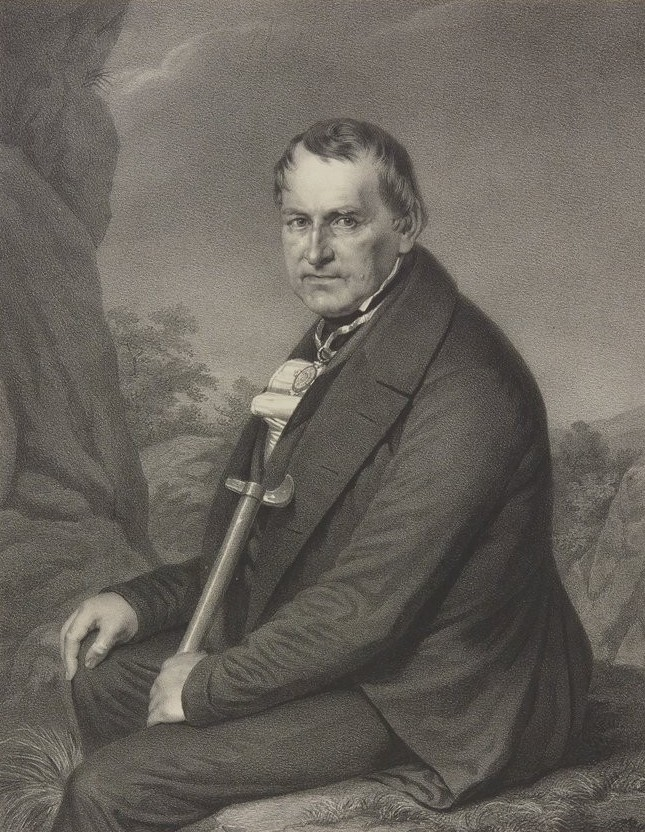
\includegraphics[width=.5\textwidth]{../../pictures/Leopold_von_Buch_btv1b105009064_(cropped).jpg}
      \end{center}
      \caption{
         {
            \small Christian Leopold von Buch (1774 -- 1853) was a German
               geologist and paleontologist. (From
               \href{https://en.wikipedia.org/wiki/Christian_Leopold_von_Buch}{Wikipedia}). Image: Lithograph by C.
               Fischer based on a painting by Carl Joseph Begas, 1850. Public domain.
         }
      }
      \vspace{-1.3cm}
   \end{center}
\end{wrapfigure}

Physical astronomy presents us with other phenomena, which cannot be fully comprehended in all their vastness without a previous acquirement of general views regarding the forces that govern the universe. Such, for instance, are the innumerable double stars, or rather suns, which revolve round one common center of gravity, and thus reveal in distant worlds the existence of the Newtonian law; the larger or smaller number of spots upon the sun, that is to say, the openings formed through the luminous and opaque atmosphere surrounding the solid nucleus; and the regular appearance, about the 13th of November and the 11th of August, of shooting stars, which probably form part of a belt of asteroids, intersecting the earth's orbit, and moving with planetary velocity.

Descending from the celestial regions to the earth, we would fain inquire into the relations that exist between the oscillations of the pendulum in air (the theory of which has been perfected by Bessel) and the density of our planet; and how the pendulum, acting the part of a plummet, can, to a certain extent, throw light upon the geological constitution of strata at great depths. By means of this instrument, we are enabled to trace the striking analogy which exists between the formation of the granular rocks composing the lava currents ejected from active volcanoes, and those endogenous masses of granite, porphyry, and serpentine, which, issuing from the interior of the earth, have broken, as eruptive rocks, through the secondary strata, and modified them by contact, either in rendering them harder by the introduction of silex, or reducing them into dolomite, or, finally, by inducing within them the formation of crystals of the most varied composition. The elevation of sporadic islands, of domes of trachyte, and cones of basalt, by the elastic forces emanating from the fluid interior of our globe, has led one of the first geologists of the age, Leopold von Buch, to the theory of the elevation of continents, and of mountain chains generally. This action of subterranean forces in breaking through and elevating strata of sedimentary rocks, of which the coast of Chile, in consequence of a great earthquake, furnished a recent example, leads to the assumption that the pelagic shells found by M. Bonpland and myself on the ridge of the Andes, at an elevation of more than 15,000 English feet, may have been conveyed to so extraordinary a position, not by a rising of the ocean, but by the agency of volcanic forces capable of elevating into ridges the softened crust of the earth. 

I apply the term volcanic, in the widest sense of the word, to every action exercised by the interior of a planet on its external crust. The surface of our globe, and that of the moon, manifest traces of this action, which in the former, at least, has varied during the course of ages. Those who are ignorant of the fact that the internal heat of the earth increases so rapidly with the increase of depth that granite is in a state of fusion about twenty or thirty geographical miles below the surface,\footnote{The determinations usually given of the point of fusion are in general much too high for refracting substances. According to the very accurate researches of Mitscherlich, the melting point of granite can hardly exceed 2372°F.

[Dr. Mantell states in The Wonders of Geology, 1848, vol. i., p. 34, that this increase of temperature amounts to 1°F for every fifty-four feet of vertical depth.] -- Tr.
} cannot have a clear conception of the causes, and the simultaneous occurrence of volcanic eruptions at places widely removed from one another, or of the extent and intersection of circles of commotion in earthquakes, or of the uniformity of temperature, and equality of chemical composition observed in thermal springs during a long course of years. The quantity of heat peculiar to a planet is, however, a matter of such importance being the result of its primitive condensation, and varying according to the nature and duration of the radiation that the study of this subject may throw some degree of light on the history of the atmosphere, and the distribution of the organic bodies embedded in the solid crust of the earth. This study enables us to understand how a tropical temperature, independent of latitude (that is, of the distance from the poles), may have been produced by deep fissures remaining open, and exhaling heat from the interior of the globe, at a period when the earth's crust was still furrowed and rent, and only in a state of semi-solidification; and a primordial condition is thus revealed to us, in which the temperature of the atmosphere, and climates generally, were owing rather to a liberation of caloric and of different gaseous emanations (that is to say, rather to the energetic reaction of the interior on the exterior) than to the position of the earth with respect to the central body, the sun.

The cold regions of the earth contain, deposited in sedimentary strata, the products of tropical climates; thus, in the coal formations, we find the trunks of palms standing upright amid conifer, tree ferns, goniatites, and fishes having rhomboidal osseous scales;\footnote{See the classical work on the fishes of the Old World by Agassiz, Rech. sur les Poissons Fossiles, 1834, vol. i., p. 38; vol. ii., p. 3, 28, 34, App., p. 6. The whole genus of Amblypterus, Ag., nearly allied to Palaeoniscus (called also Paleothrissum), lies buried beneath the Jura formations in the old carboniferous strata. Scales which, in some fishes, as in the family of Lepidoides (order of Ganoides), are formed like teeth and covered in certain parts with enamel, belong, after the Placoides, to the oldest forms of fossil fishes; their living representatives are still found in two genera, the Bichir of the Nile and Senegal, and the Lepidosteus of the Ohio.} in the Jura limestone, colossal skeletons of crocodiles, plesiosaurs, planulites, and stems of the cycads; in the chalk formations, small polythalamia and bryozoa, whose species still exist in our seas; in tripoli, or polishing slate, in the semiopal and the farinaceous opal or mountain meal, agglomerations of siliceous infusoria, which have been brought to light by the powerful microscope of Ehrenberg;\footnote{[The polishing slate of Bilin is stated by M. Ehrenberg to formaseries of strata fourteen feet in thickness, entirely made up of the siliccous shells of Gaillonelle, of such extreme minuteness that a cubicinch of the stone contains fortyone thousand millions The Bergmeht(mountain meal or fossil farina) of San Fiora, in Tuscany, is one masaof animalculites. See the interesting work of G. A, Mantell, On teeMedals of Creation, vol. i., p. 223.] -- Tr.} and, lastly, in transported soils, and in certain caves, the bones of elephants, hyenas, and lions. An intimate acquaintance with the physical phenomena of the universe leads us to regard the products of warm latitudes that are thus found in a fossil condition in northern regions not merely as incentives to barren curiosity, but as subjects awakening deep reflection and opening new sources of study.

The number and the variety of the objects I have alluded to give rise to the question of whether general considerations of physical phenomena can be made sufficiently clear to persons who have not acquired a detailed and special knowledge of descriptive natural history, geology, or mathematical astronomy. I think we ought to distinguish here between him whose task it is to collect the individual details of various observations and study the mutual relations existing among them, and him to whom these relations are to be revealed under the form of general results. The former should be acquainted with the specialties of phenomena, that he may arrive at a generalization of ideas as the result, at least in part, of his own observations, experiments, and calculations. It cannot be denied that where there is an absence of positive knowledge of physical phenomena, the general results which impart so great a charm to the study of nature cannot all be made equally clear and intelligible to the reader. But still, I venture to hope that in the work which I am now preparing on the physical laws of the universe, the greater part of the facts advanced can be made manifest without the necessity of appealing to fundamental views and principles. The picture of nature thus drawn, notwithstanding the want of distinctness of some of its outlines, will not be the less able to enrich the intellect, enlarge the sphere of ideas, and nourish and vivify the imagination.

There is, perhaps, some truth in the accusation advanced against many German scientific works, that they lessen the value of general views by an accumulation of detail, and do not sufficiently distinguish between those great results which form, as it were, the beacon lights of science, and the long series of means by which they have been attained. This method of treating scientific subjects led the most illustrious of our poets\footnote{G\"oethe, in Die Aphorismen uber Naturwissenschaft, bd. l.. 8. 155 (Werke kleine Ausgabe, von 1833.)} to exclaim, with impatience, "The Germans have the art of making science inaccessible." An edifice cannot produce a striking effect until the scaffolding is removed, that had of necessity been used during its erection. Thus the uniformity of figure observed in the distribution of continental masses, which all terminate toward the south in a pyramidal form, and expand toward the north (a law that determines the nature of climates, the direction of currents in the ocean and the atmosphere, and the transition of certain types of tropical vegetation toward the southern temperate zone), may be clearly apprehended without any knowledge of the geodesical and astronomical operations by means of which these pyramidal forms of continents have been determined. In like manner, physical geography teaches us by how many leagues the equatorial axis exceeds the polar axis of the globe, and shows us the mean equality of the flattening of the two hemispheres, without entailing on us the necessity of giving the detail of the measurement of the degrees in the meridian, or the observations on the pendulum, which have led us to know that the true figure of our globe is not exactly that of a regular ellipsoid of revolution, and that this irregularity is reflected in the corresponding irregularity of the movements of the moon.

The views of comparative geography have been specially enlarged by that admirable work, Erdkunde im Verhältniss zur Natur und zur Geschichte, in which Carl Ritter so ably delineates the physiognomy of our globe, and shows the influence of its external configuration on the physical phenomena on its surface, on the migrations, laws, and manners of nations, and on all the principal historical events enacted upon the face of the earth.

France possesses an immortal work, L'Exposition du Système du Monde, in which the author has combined the results of the highest astronomical and mathematical labors, and presented them to his readers free from all processes of demonstration. The structure of the heavens is here reduced to the simple solution of a great problem in mechanics; yet Laplace's work has never yet been accused of incompleteness and want of profundity.

The distinction between dissimilar subjects, and the separation of the general from the special, are not only conduciveto the attainment of perspicuity in the composition of a physial history of the universe, but are also the means by whicha character of greater elevation may be imparted to the studyof nature. By the suppression of all unnecessary detail, thegreat masses are better seen, and the reasoning faculty is enabled to grasp all that might otherwise escape the limited rangeof the senses.

The exposition of general results has, it must be owned, been singularly facilitated by the happy revolution experienced since the close of the last century, in the condition of all the special sciences, more particularly of geology, chemistry, and descriptive natural history. In proportion as laws admit of more general application, and as sciences mutually enrich each other, and by their extension become connected together in more numerous and more intimate relations, the development of general truths may be given with conciseness devoid of superficiality. On being first examined, all phenomena appear to be imagined, and it is only by the result of a multiplicity of observations, combined by reason, that we are able to trace the mutual relations existing between them. If, however, in the present age, which is so strongly characterized by a brilliant course of scientific discoveries, we perceive a want of connection in the phenomena of certain sciences, we may anticipate the revelation of new facts, whose importance will probably be commensurate with the attention directed to these branches of study. Expectations of this nature may be entertained with regard to meteorology, several parts of optics, and to radiating heat, and electromagnetism, since the admirable discoveries of Melloni and Faraday. A fertile field is here opened to discovery, although the voltaic pile has already taught us the intimate connection existing between electric, magnetic, and chemical phenomena. Who will venture to affirm that we have any precise knowledge, in the present day, of that part of the atmosphere which is not oxygen, or that thousands of gaseous substances affecting our organs may not be mixed with the nitrogen, or, finally, that we have even discovered the whole number of the forces which pervade the universe?

It is not the purpose of this essay on the physical history of the world to reduce all sensible phenomena to a small number of abstract principles, based on reason only. The physical history of the universe, whose exposition I attempt to develop, does not pretend to rise to the perilous abstractions of a purely rational science of nature, and is simply a physical geography, combined with a description of the regions of space and the bodies occupying them. Devoid of the profoundness of a purely speculative philosophy, my essay on the Cosmos treats of the contemplation of the universe, and is based upon a rationalempiricism, that is to say, upon the results of the facts registered by science, and tested by the operations of the intellect. It is within these limits alone that the work, which I now venture to undertake, appertains to the sphere of labor to which I have devoted myself throughout the course of my long scientific career. The path of inquiry is not unknown to me, although it may be pursued by others with greater success. The unity which I seek to attain in the development of the great phenomena of the universe is analogous to that which historical composition is capable of acquiring. All points relating to the accidental individualities, and the essential variations of the actual, whether in the form and arrangement of natural objects in the struggle of man against the elements, or of nations against nations, do not admit of being based only on a rational foundation, that is to say, of being deduced from ideas alone.

It seems to me that a like degree of empiricism attaches to the Description of the Universe and to Civil History; but in reflecting upon physical phenomena and events, and tracing their causes by the process of reason, we become more and more convinced of the truth of the ancient doctrine, that the forces inherent in matter, and those which govern the moral world, exercise their action under the control of primordial necessity, and in accordance with movements occurring periodically after longer or shorter intervals.

It is this necessity, this occult but permanent connection, this periodical recurrence in the progressive development of forms, phenomena, and events, which constitute nature, obedient to the first impulse imparted to it. Physics, as the term signifies, is limited to the explanation of the phenomena of the material world by the properties of matter. The ultimate object of the experimental sciences is, therefore, to discover laws, and to trace their progressive generalization. All that exceeds this goes beyond the province of the physical description of the universe and appertains to a range of higher speculative views.

Emanuel Kant, one of the few philosophers who have escaped the imputation of impiety, has defined with rare sagacity the limits of physical explanations, in his celebrated essay "On the Theory and Structure of the Heavens", published at Königsberg in 1755.

The study of a science that promises to lead us through the vast range of creation may be compared to a journey in a far distant land. Before we set forth, we consider, and often with distrust, our own strength, and that of the guide we have chosen. But the apprehensions which have originated in the abundance and the difficulties attached to the subjects we would embrace recede from view as we remember that with the increase of observations in the present day there has also arisen a more intimate knowledge of the connection existing among all phenomena. It has not unfrequently happened that the researches made at remote distances have often and unexpectedly thrown light upon subjects which had long resisted the attempts made to explain them within the narrow limits of our own sphere of observation. Organic forms that had long remained isolated, both in the animal and vegetable kingdom, have been connected by the discovery of intermediate links or stages of transition. The geography of beings endowed with life attains completeness as we see the species, genera, and entire families belonging to one hemisphere, reflected, as it were, in analogous animal and vegetable forms in the opposite hemisphere. These are, so to speak, the equivalents which mutually personate and replace one another in the great series of organisms. These connecting links and stages of transition may be traced, alternately, in a deficiency or an excess of development of certain parts, in the mode of junction of distinct organs, in the differences in the balance of forces, or in a resemblance to intermediate forms, which are not permanent, but merely characteristic of certain phases of normal development. Passing from the consideration of beings endowed with life to that of inorganic bodies, we find many striking illustrations of the high state of advancement to which modern geology has attained. We thus see, according to the grand views of Elie de Beaumont, how chains of mountains dividing different climates and floras and different races of men reveal to us their relative age, both by the character of the sedimentary strata they have uplifted, and by the directions which they follow over the long fissures with which the earth's crust is furrowed. Relations of superposition of trachyte and of syenitic porphyry, of diorite and of serpentine, which remain doubtful when considered in the auriferous soil of Hungary in the rich platinum districts of the Ural, and on the southwestern declivity of the Siberian Altai, are elucidated by the observations that have been made on the plateaus of Mexico and Antioquia, and in the unhealthy ravines of Choco. The most important facts on which the physical history of the world has been based in modern times have not been accumulated by chance. It has at length been fully acknowledged, and the conviction is characteristic of the age, that the narratives of distant travels, too long occupied in the mere recital of hazardous adventures, can only be made a source of instruction where the traveler is acquainted with the condition of the science he would enlarge and is guided by reason in his researches.

It is by this tendency to generalization, which is only dangerous in its abuse, that a great portion of the physical knowledge already acquired may be made the common property of all classes of society; but, in order to render the instruction imparted by these means commensurate with the importance of the subject, it is desirable to deviate as widely as possible from the imperfect compilations designated, till the close of the eighteenth century, by the inappropriate term of popular knowledge. I take pleasure in persuading myself that scientific subjects may be treated of in language at once dignified, grave, and animated, and that those who are restricted within the circumscribed limits of ordinary life, and have long remained strangers to an intimate communion with nature, may thus have opened to them one of the richest sources of enjoyment, by which the mind is invigorated by the acquisition of new ideas. Communion with nature awakens within us perceptive faculties that had long lain dormant; and we thus comprehend at a single glance the influence exercised by physical discoveries on the enlargement of the sphere of intellect, and perceive how a judicious application of mechanics, chemistry, and other sciences may be made conducive to national prosperity.

A more accurate knowledge of the connection of physical phenomena will also tend to remove the prevalent error that all branches of natural science are not equally important in relation to general cultivation and industrial progress. An arbitrary distinction is frequently made between the various degrees of importance appertaining to mathematical sciences, to the study of organized beings, the knowledge of electromagnetism, and investigations of the general properties of matter in its different conditions of molecular aggregation; and it is not uncommon presumptuously to affix a supposed stigma upon researches of this nature, by terming them purely theoretical, forgetting, although the fact has been long attested, that in the observation of a phenomenon, which at first sight appears to be wholly isolated, may be concealed the germ of a great discovery. When Aloysio Galvani first stimulated the nervous fiber by the accidental contact of two heterogeneous metals, his contemporaries could never have anticipated that the action of the voltaic pile would discover to us, in the alkalies, metals of a silvery luster, so light as to swim on water, and eminently inflammable; or that it would become a powerful instrument of chemical analysis, and at the same time a thermoscope and a magnet. When Huygens first observed, in 1678, the phenomenon of the polarization of light, exhibited in the difference between the two rays into which a pencil of light divides itself in passing through a doubly refracting crystal, it could not have been foreseen that, a century and a half later, the great philosopher Arago would, by his discovery of chromatic polarization, be led to discern, by means of a small fragment of Iceland spar, whether solar light emanates from a solid body or a gaseous covering, or whether comets transmit light directly or merely by reflection.\footnote{Aragos Discoveries in the year 1811.Delambres Histoire de Ast., p. 652. (Passage already quoted.)}

An equal appreciation of all branches of the mathematical, physical, and natural sciences is a special requirement of the present age, in which the material wealth and the growing prosperity of nations are principally based upon a more enlightened employment of the products and forces of nature. The most superficial glance at the present condition of Europe reveals that a diminution, or even a total annihilation of national prosperity, must be the award of those states who shrink with slothful indifference from the great struggle of rival nations in the career of the industrial arts. It is with nations as with nature, which, according to a happy expression of G\"oethe\footnote{G\"oethe, in Die Aphorismen über Naturwissenschaft. Werke, bd. 1.,a4}, "knows no pause in progress and development, and attaches her curse on all inaction". The propagation of an earnest and sound knowledge of science can therefore alone avert the dangers of which I have spoken. Man cannot act upon nature, or appropriate her forces to his own use, without comprehending their full extent, and having an intimate acquaintance with the laws of the physical world. Bacon has said that, in human societies, knowledge is power. Both must rise and sink together. But the knowledge that results from the free action of thought is at once the delight and the indestructible prerogative of man; and in forming part of the wealth of mankind, it not unfrequently serves as a substitute for the natural riches, which are but sparingly scattered over the earth. Those states which take no active part in the general industrial movement, in the choice and preparation of natural substances, or in the application of mechanics and chemistry, and among whom this activity is not appreciated by all classes of society, will infallibly see their prosperity diminish in proportion as neighboring countries become strengthened and invigorated under the genial influence of arts and sciences.

As in nobler spheres of thought and sentiment, in philosophy, poetry, and the fine arts, the object at which we aim ought to be an inward one - an ennoblement of the intellect. So ought we likewise, in our pursuit of science, to strive after a knowledge of the laws and the principles of unity that pervade the vital forces of the universe; and it is by such a course that physical studies may be made subservient to the progress of industry, which is a conquest of mind over matter. By a happy connection of causes and effects, we often see the useful linked to the beautiful and the exalted. The improvement of agriculture in the hands of freemen, and on properties of a moderate extent, the flourishing state of the mechanical arts freed from the trammels of municipal restrictions, the increased impetus imparted to commerce by the multiplied means of contact of nations with each other, are all brilliant results of the intellectual progress of mankind, and of the amelioration of political institutions, in which this progress is reflected. The picture presented by modern history ought to convince those who are tardy in awakening to the truth of the lesson it teaches.

Nor let it be feared that the marked predilection for thestudy of nature, and for industrial progress, which is so characteristic of the present age, should necessarily have a tendency to retard the noble exertions of the intellect in the domainsof philosophy, classical history, and antiquity, or to deprivethe arts by which life is embellished of the vivifying breath of.magination. Where all the germs of civilization are developed beneath the wgis of free institutions and wise legislation,there is no cause for apprehending that any one branch ofsnowledge should be cultivated to the prejudice of others.All afford the state precious fruits, whether they yield nourishment to man and constitute his physical wealth, or whether,more permanent in their nature, they transmit in the works .of mind the glory of nations to remotest posterity. The Spartans, notwithstanding their Doric austerity, prayed the godsto grant them ``the beautiful with the good.''\footnote{Pseudo-Plato.Alcib., xi., p. 184, ed. Steph.; Plut., Instituta Laconica, p. 253, ed. Hutten.}

I will no longer dwell upon the considerations of the influence exercised by the mathematical and physical sciences on all that appertains to the material wants of social life, for the vast extent of the course on which I am entering forbids me to insist further upon the utility of these applications. Accustomed to distant excursions, I may, perhaps, have erred in describing the path before us as more smooth and pleasant than it really is, for such is wont to be the practice of those who delight in guiding others to the summits of lofty mountains; they praise the view even when a great part of the distant plains lie hidden by clouds, knowing that this half-transparent vapory veil imparts to the scene a certain charm from the power exercised by the imagination over the domain of the senses. In like manner, from the height occupied by the physical history of the world, all parts of the horizon will not appear equally clear and well defined. This indistinctness will not, however, be wholly owing to the present imperfect state of some of the sciences, but in part, likewise, to the unskillfulness of the guide who has imprudently ventured to ascend these lofty summits.

The object of this introductory notice is not, however, solely to draw attention to the importance and greatness of the physical history of the universe, for in the present day these are too well understood to be contested, but likewise to prove how, without detriment to the stability of special studies, we may be enabled to generalize our ideas by concentrating them in one common focus, and thus arrive at a point of view from which all the organisms and forces of nature may be seen as one living, active whole, animated by one sole impulse. ``Nature, as Schelling remarks in his poetic discourse on art, is not an inert mass; and to him who can comprehend her vast sublimity, she reveals herself as the creative force of the universe before all time, eternal, ever active, she calls to life all things, whether perishable or imperishable.''

By uniting, under one point of view, both the phenomena of our own globe and those presented in the regions of space, we embrace the limits of the science of the Cosmos, and convert the physical history of the globe into the physical history of the universe, the one term being modeled upon that of the other. This science of the Cosmos is not, however, to be regarded as a mere encyclopedic aggregation of the most important and general results that have been collected together from special branches of knowledge. These results are nothing more than the materials for a vast edifice, and their combination can not constitute the physical history of the world, whose exalted part it is to show the simultaneous action and the connecting links of the forces which pervade the universe. The distribution of organic types in different climates and at different elevations - that is to say, the geography of plants and animals - differs as widely from botany and descriptive zoology as geology does from mineralogy, properly so called. The physical history of the universe must not, therefore, be confounded with the encyclopedias of the Natural Sciences, as they have hitherto been compiled, and whose title is as vague as their limits are ill defined. In the work before us, partial facts will be considered only in relation to the whole.

The higher the point of view, the greater is the necessity for a systematic mode of treating the subject in language at once animated and picturesque.

But thought and language have ever been most intimately allied. If language, by its originality of structure and its native richness, can, in its delineations, interpret thought with grace and clearness, and if, by its happy flexibility, it can paint with vivid truthfulness the objects of the external world; it reacts at the same time upon thought, and animates it, as it were, with the breath of life. It is this mutual reaction which makes words more than mere signs and forms of thought; and the beneficent influence of a language is most strikingly manifested on its native soil, where it has sprung spontaneously from the minds of the people, whose character it embodies. Proud of a country that seeks to concentrate her strength in intellectual unity, the writer recalls with delight the advantages he has enjoyed in being permitted to express his thoughts in his native language; and truly happy is he who, in attempting to give a lucid exposition of the great phenomena of the universe, is able to draw from the depths of a language, which, through the free exercise of thought, and by the effusions of creative fancy, has for centuries past exercised so powerful an influence over the destinies of man.

\section[Limits and Method of Exposition ...]{Limits and Method of Exposition of the Physical Description of the Universe.}

I have endeavored, in the preceding part of my work, to explain and illustrate, by various examples, how the enjoyments presented by the aspect of nature, varying as they do in the sources from whence they flow, may be multiplied and ennobled by an acquaintance with the connection of phenomena and the laws by which they are regulated. It remains, then, for me to examine the spirit of the method in which the exposition of the physical description of the universe should be conducted, and to indicate the limits of this science in accordance with the views I have acquired in the course of my studies and travels in various parts of the earth. I trust I may flatter myself with a hope that a treatise of this nature will justify the title I have ventured to adopt for my work, and exonerate me from the reproach of a presumption that would be doubly reprehensible in a scientific discussion.

Before entering upon the delineation of the partial phenomena which are found to be distributed in various groups, I would consider a few general questions intimately connected together, and bearing upon the nature of our knowledge of the external world and its different relations, in all epochs of history and in all phases of intellectual advancement. Under this head will be comprised the following considerations:

\begin{enumerate}

\item The precise limits of the physical description of the universe, considered as a distinct science.

\item A brief enumeration of the totality of natural phenomena, presented under the form of a general delineation of nature.

\item The influence of the external world on the imagination and feelings, which has acted in modern times as a powerful impulse toward the study of natural science, by giving animation to the description of distant regions and to the delineation of natural scenery, as far as it is characterized by vegetable physiognomy and by the cultivation of exotic plants, and their arrangement in well-contrasted groups.

\item The history of the contemplation of nature, or the progressive development of the idea of the Cosmos, considered with reference to the historical and geographical facts that have led to the discovery of the connection of phenomena.

\end{enumerate}

The higher the point of view from which natural phenomena may be considered, the more necessary it is to circumscribe the science within its just limits, and to distinguish it from all other analogous or auxiliary studies.

Physical cosmography is founded on the contemplation of all created things - all that exists in space, whether as substances or forces - that is, all the material beings that constitute the universe. The science which I would attempt to define presents itself, therefore, to man, as the inhabitant of the earth, under a twofold form: as the earth itself and the regions of space. It is with a view of showing the actual character and the independence of the study of physical cosmography, and at the same time indicating the nature of its relations to general physics, descriptive natural history, geology, and comparative geography, that I will pause for a few moments to consider that portion of the science of the Cosmos which concerns the earth. As the history of philosophy does not consist of a mere material enumeration of the philosophical views entertained in different ages, neither should the physical description of the universe be a simple encyclopedic compilation of the sciences we have enumerated. The difficulty of defining the limits of intimately connected studies has been increased, because for centuries it has been customary to designate various branches of empirical knowledge by terms which admit either too wide or too limited a definition of the ideas which they were intended to convey, and are, besides, objectionable from having had a different signification in those classical languages of antiquity from which they have been borrowed. The terms physiology, physics, natural history, geology, and geography arose, and were commonly used, long before clear ideas were entertained of the diversity of objects embraced by these sciences, and consequently of their reciprocal limitation. Such is the influence of long habit upon language, that by one of the nations of Europe most advanced in civilization the word "physic" is applied to medicine, while in a society of justly deserved universal reputation, technical chemistry, geology, and astronomy (purely experimental sciences) are comprised under the head of "Philosophical Transactions."

An attempt has often been made, and almost always in vain,to substitute new and more appropriate terms for these ancientdesignations, which, notwithstanding their undoubted vaguehess, are now generally understood. These changes have beenproposed, for the most part, by those who have occupied themselves with the general classification of the various branchesof knowledge, from the first appearance of the great encyclopedia (Margarita Philosophica) of Gregory Reisch,\footnote{The Margarita Philosophica of Gregory Reisch, prior of the Chartreuse at Freiburg, first appeared under the following title Zpitomeomnis Philosophie, alias Margarita Philosophica, tractans de omni generiscibili. The Heidelberg edition (1486), and that of Strasburg (1504),both bear this title, but the first part was suppressed in the Freiburgedition of the same year, as well as in the twelve subsequent editions,which succeeded one another, at short intervals, till 1535. This workexercised a great influence on the diffusion of mathematical and physical sciences toward the beginning of the sixteenth century, and Unasles,the learned author of L'Apergu Historique des M\'{e}thodes en G\'{e}om\'{e}ire(1837), has shown the great importance of Reischs Encyclopedia inthe history of mathematics in the Middle Ages. I have had recourseto a passage in the Margarita Philosophica, found only in the editionof 1513, to elucidate the important question of the relations betweenthe statements of the geographer of SaintDie, Hylacomilus (MartinWaldseemiiller), the first who gave the name of America to the NewContinent, and those of Amerigo Vespucci, Ren\'{e}, King of Jerusalemand Duke of Lorraine, as also those contained in the celebrated editionsof Ptolemy of 1513 and 1522. See my Examen Critique de la G\'{e}ographie du Nouveau Continent, et des Progr\'{e}s de l Astronomie Nautiqueauz 15e et 16e Si\'{e}cles, t. iv., p. 99125.} prior ofthe Chartreuse at Freiburg, toward the close of the fifteenthcentury, to Lord Bacon, and from Bacon to DAlembert ; andin recent times to an eminent physicist, Andr\'{e} Marie Amp\'{e}re.\footnote{Amp\'{e}re, Essai sur la Phil. des Sciences, 1834, p. 25. Whewell, Philosophy of the Inductive Sciences, vol, ii., p. 277. Park, Pantology p. 87}

The selection of an inappropriate Greek nomenclature has perhaps been even more prejudicial to the last of these attemptsthan the injudicious use of binary divisions and the excessivetnultiplication.of groups.

The physical description of the world, considering the universe as an object of the external senses, does undoubtedly require the aid of general physics and of descriptive natural history, but the contemplation of all created things, which are linked together, and form one whole, animated by internal forces, gives to the science we are considering a peculiar character. Physical science considers only the general properties of bodies; it is the product of abstraction, a generalization of perceptible phenomena; and even in the work in which were laid the first foundations of general physics, in the eight books on physics of Aristotle,\footnote{All changes in the physical world may be reduced to motion. Aristot., Phys. Ausc., iii., 1 and 4, p. 200, 201. Bekker, viii., 1, 8, and D, p. 250, 262, 265. De Genere et Corr., ii., 10, p. 336. PseudoAristot., De Mundo. ynp. vi., p. 398.} all the phenomena of nature are considered as depending upon the primitive and vital action of one sole force, from which emanate all the movements of the universe. The terrestrial portion of physical cosmography, for which I would willingly retain the expressive designation of physical geography, treats of the distribution of magnetism in our planet with relation to its intensity and direction, but does not enter into a consideration of the laws of attraction or repulsion of the poles, or the means of eliciting either permanent or transitory electromagnetic currents. Physical geography depicts in broad outlines the even or irregular configuration of continents, the relations of superficial area, and the distribution of continental masses in the two hemispheres, a distribution which exercises a powerful influence on the diversity of climate and the meteorological modifications of the atmosphere; this science defines the character of mountain chains, which, having been elevated at different epochs, constitute distinct systems, whether they run in parallel lines or intersect one another; determines the mean height of continents above the level of the sea, the position of the center of gravity of their volume, and the relation of the highest summits of mountain chains to the mean elevation of their crests, or to their proximity with the seashore. It depicts the eruptive rocks as principles of movement, acting upon the sedimentary rocks by traversing, uplifting, and inclining them at various angles; it considers volcanoes either as isolated, or ranged in single or indouble series, and extending their sphere of action to various distances, either by raising long and narrow lines of rocks, or by means of circles of commotion, which expand or diminish in diameter in the course of ages. This terrestrial portion of the science of the Cosmos describes the strife of the liquid element with the solid land; it indicates the features possessed in common by all great rivers in the upper and lower portion of their course, and in their mode of bifurcation when their basins are unclosed; and shows us rivers breaking through the highest mountain chains, or following for a long time course parallel to them, either at their base, or at a considerable distance, where the elevation of the strata of the mountain system and the direction of their inclination correspond to the configuration of the tableland. It is only the general results of comparative orography and hydrography that belong to the science whose true limits I am desirous of determining and not the special enumeration of the greatest elevations of our globe, of active volcanoes, of rivers, and the number of their tributaries, these details falling rather within the domain of geography, properly so called. We would here only consider phenomena in their mutual connection, and in their relations to different zones of our planet, and to its physical constitution generally. The specialties both of inorganic and organized matter, classed according to analogy of form and composition, undoubtedly constitute a most interesting branch of study, but they appertain to a sphere of ideas having no affinity with the subject of this work.

The description of different countries certainly furnishes us with the most important materials for the composition of a physical geography; but the combination of these different descriptions, ranged in series, would as little give us a true image of the general conformation of the irregular surface of our globe, as a succession of all the floras of different regions would constitute that which I designate as a Geography of Plants. It is by subjecting isolated observations to the process of thought, and by combining and comparing them, that we are enabled to discover the relations existing in common between the climatic distribution of beings and the individuality of organic forms (in the morphology or descriptive natural history of plants and animals); and it is by induction that we are led to comprehend numerical laws, the proportion of natural families to the whole number of species, and to designate the latitude or geographical position of the zones in whose plains each organic form attains the maximum of its development. Considerations of this nature, by their tendency to generalization, impress a nobler character on the physical description of the globe, and enable us to understand how the aspect of the scenery, that is to say, the impression produced upon the mind by the physiognomy of the vegetation, depends upon the local distribution, the number, and the luxuriance of growth of the vegetable forms predominating in the general mass. The catalogues of organized beings, to which was formerly given the pompous title of Systems of Nature, present us with an admirably connected arrangement by analogies of structure, either in the perfected development of these beings, or in the different phases which, in accordance with the views of a spiral evolution, affect in vegetables the leaves, bracts, calyx, corolla, and fructifying organs; and in animals, with more or less symmetrical regularity, the cellular and fibrous tissues, and their perfect or but obscurely developed articulations. But these pretended systems of nature, however ingenious their mode of classification may be, do not show us organic beings as they are distributed in groups throughout our planet, according to their different relations of latitude and elevation above the level of the sea, and to climatic influences, which are owing to general and often very remote causes. The ultimate aim of physical geography is, however, as we have already said, to recognize unity in the vast diversity of phenomena, and by the exercise of thought and the combination of observations, to discern the constancy of phenomena in the midst of apparent changes. In the exposition of the terrestrial portion of the Cosmos, it will occasionally be necessary to descend to very special facts; but this will only be in order to recall the connection existing between the actual distribution of organic beings over the globe, and the laws of the ideal classification by natural families, analogy of internal organization, and progressive evolution.

It follows from these discussions on the limits of the various sciences, and more particularly from the distinction which must necessarily be made between descriptive botany (morphology of vegetables) and the geography of plants, that in the physical history of the globe, the innumerable multitude of organized bodies which embellish creation are considered rather according to zones of habitation or stations, and to differently inflected isothermal bands, than with reference to the principles of gradation in the development of internal organism. Notwithstanding this, botany and zoology, which constitute the natural history of all organized beings, are the fruitful sources whence we draw the materials necessary to give a solid basis to the study of the mutual relations and connection of phenomena.

We will here subjoin one important observation by way of elucidating the connection of which we have spoken. The first general glance over the vegetation of a vast extent of a continent shows us forms the most dissimilar - Graminee and Orchidex, Conifere and oaks, in local approximation to one another; while natural families and genera, instead of being locally associated, are dispersed as if by chance. This dispersion is, however, only apparent. The physical description of the globe teaches us that vegetation everywhere presents numerically constant relations in the development of its forms and types; that in the same climates, the species which are wanting in one country are replaced in a neighboring one by other species of the same family; and that this law of substitution, which seems to depend upon some inherent mysteries of the organism, considered with reference to its origin, maintains in contiguous regions a numerical relation between the species of various great families and the general mass of the phanerogamic plants constituting the two floras. We thus find a principle of unity and a primitive plan of distribution revealed in the multiplicity of the distinct organizations by which these regions are occupied; and we also discover in each zone, and diversified according to the families of plants, a slow but continuous action on the aerial ocean, depending upon the influence of light -- the primary condition of all organic vitality -- on the solid and liquid surface of our planet. It might be said, in accordance with a beautiful expression of Lavoisier, that the ancient marvel of the myth of Prometheus was incessantly renewed before our eyes.

If we extend the course which we have proposed, following in the exposition of the physical description of the earth to the sidereal part of the science of the Cosmos, the delineation of the regions of space and the bodies by which they are occupied, we shall find our task simplified in no common degree. If, according to ancient but unphilosophical forms of nomenclature, we would distinguish between physics, that is to say, general considerations on the essence of matter, and the forces by which it is actuated, and chemistry, which treats of the nature of substances, their elementary composition, and those attractions that are not determined solely by the relations of mass, we must admit that the description of the earth comprises at once physical and chemical actions. In addition to gravitation, which must be considered as a primitive force in nature, we observe that attractions of another kind are at work around us, both in the interior of our planet and on its surface. These forces, to which we apply the term chemical affinity, act upon molecules in contact, or at infinitely minute distances from one another,\footnote{On the question already discussed by Newton, regarding the difference existing between the attraction of masses and molecular attraction, see Laplace, Exposition du Syst\'{e}me du Monde, p. 384, and supplementto book x. of the Mecanique C\'{e}leste, p, 3, 4; Kant, Metaph. Agfangsgrinde der Naturwissenschaft, Sam. Werke, 1839, bd. v., s. 309 (Metaphysical Principles of the Nataral Sciences); Pectet, Physique, 1838.vol. i., p. 5963} and which, being differently modified by electricity, heat, condensation in porous bodies, or by the contact of an intermediate substance, animate equally the inorganic world and animal and vegetable tissues. If we except the small asteroids, which appear to us under the forms of a\'{e}rolites and shooting stars, the regions of space have hitherto presented to our direct observation physical phenomena alone; and in the case of these, we know only with certainty the effects depending upon the quantitative relations of matter or the distribution of masses. The phenomena of the regions of space may consequently be considered as influenced by simple dynamics laws - the laws of motion.

The effects that may arise from the specific difference and the heterogeneous nature of matter have not hitherto entered into our calculations of the mechanism of the heavens. The only means by which the inhabitants of our planet can enter into relation with the matter contained within the regions of space, whether existing in scattered forms or united into large spheroids, is by the phenomena of light, the propagation of luminous waves, and by the influence universally exercised by the force of gravitation or the attraction of masses. The existence of a periodical action of the sun and moon on the variations of terrestrial magnetism is even at the present day extremely problematical. We have no direct experimental knowledge regarding the properties and specific qualities of the masses circulating in space, or of the matter of which they are probably composed, if we except what may be derived from the fall of a\'{e}rolites or meteoric stones, which, as we have already observed, enter within the limits of our terrestrial sphere. It will be sufficient here to remark, that the direction and the excessive velocity of projection (a velocity wholly planetary) manifested by these masses, render it more than probable that they are small celestial bodies, which, being attracted by our planet, are made to deviate from their original course, and thus reach the earth enveloped in vapors, and in a high state of actual incandescence. The familiar aspect of these asteroids, and the analogies which they present with the minerals composing the earth's crust, undoubtedly afford ample grounds for surprise;\footnote{[The analysis of an a\'{e}rolite which fell a few years since in Maryland, United States, and was examined by Professor Silliman, of New Haven, Connecticut, gave the following results Oxyd of iron, 24; oxyd of nickel, 125; silica, with earthy matter, 346; sulphur, a trace2871. Dr. Mantells Wonders of Geology, 1848, vol.i., p. 51.J] -- Tr.} but, in my opinion, the only conclusion to be drawn from these facts is, that, in general, planets and other sidereal masses, which, by the influence of a central body, have been agglomerated into rings of vapor, and subsequently into spheroids, being integrant parts of the same system, and having one common origin, may likewise be composed of substances chemically identical. Again, experiments with the pendulum, particularly those prosecuted with such rare precision by Bessel, confirm the Newtonian axiom, that bodies the most heterogeneous in their nature (as water, gold, quartz, granular limestone, and different masses of a\'{e}rolites) experience a perfectly similar degree of acceleration from the attraction of the earth. To the experiments of the pendulum may be added the proofs furnished by purely astronomical observations. The almost perfect identity of the mass of Jupiter, deduced from the influence exercised by this stupendous planet on its own satellites, on Encke's comet of short period, and on the small planets Vesta, Juno, Ceres, and Pallas, indicates with equal certainty that within the limits of actual observation attraction is determined solely by the quantity of matter.\footnote{Poisson, Connaissances des Temps pour l Ann\'{e}e 1836, p. 6466.Bessel, Poggendorfs Annalen, bd. xxy.,s.417. Encke, Abhanalungender Berliner Academie (Trans. of the Berlin Academy), 1826, s. 217.Mitscherlich, Lehrbuch der Chemie (Manual of Chemistry), 1837 bd i.8. 352.}

This absence of any perceptible difference in the nature of matter, alike proved by direct observation and theoretical deductions, imparts a high degree of simplicity to the mechanism of the heavens. The immeasurable extent of the regions of space being subjected to laws of motion alone, the sidereal portion of the science of the Cosmos is based on the pure and abundant source of mathematical astronomy, as is the terrestrial portion on physics, chemistry, and organic morphology; but the domain of these three last-named sciences embraces the consideration of phenomena which are so complicated, and have, up to the present time, been found so little susceptible to the application of rigorous method, that the physical science of the earth cannot boast of the same certainty and simplicity in the exposition of facts and their mutual connection which characterize the celestial portion of the Cosmos. It is not improbable that the difference to which we allude may furnish an explanation of the cause which, in the earliest ages of intellectual culture among the Greeks, directed the natural philosophy of the Pythagoreans with more ardor to the heavenly bodies and the regions of space than to the earth and its productions, and how through Philolatis, and subsequently through the analogous views of Aristarchus of Samos, and of Seleucus of Erythrea, this science has been made more conducive to the attainment of a knowledge of the true system of the world than the natural philosophy of the Ionian school could ever be to the physical history of the earth. Giving but little attention to the properties and specific differences of matter filling space, the great Italian school, in its Doric gravity, turned by preference toward all that relates to measure, to the form of bodies, and to the number and distances of the planets,\footnote{Compare Otfried Millers Dorien, bd. i., 8. 365.} while the Ionian physicists directed their attention to the qualities of matter, its true or supposed metamorphoses, and to relations of origin. It was reserved for the powerful genius of Aristotle, alike profoundly speculative and practical, to sound with equal success the depths of abstraction and the inexhaustible resources of vital activity pervading the material world.

Several highly distinguished treatises on physical geography are prefaced by an introduction, whose purely astronomical sections are directed to the consideration of the earth in its planetary dependence, and as constituting a part of that great system which is animated by one central body, the sun. This course is diametrically opposed to the one which I propose following. In order adequately to estimate the dignity of the Cosmos, it is requisite that the sidereal portion, termed by Kant the natural history of the heavens, should not be made subordinate to the terrestrial. In the science of the Cosmos, according to the expression of Aristarchus of Samos, the pioneer of the Copernican system, the sun, with its satellites, was nothing more than one of the innumerable stars by which space is occupied. The physical history of the world must, therefore, begin with the description of the heavenly bodies, and with a geographical sketch of the universe, or, I would rather say, a true map of the world, such as was traced by the bold hand of the elder Herschel. If, notwithstanding the smallness of our planet, the most considerable space and the most attentive consideration be here afforded to that which exclusively concerns it, this arises solely from the disproportion in the extent of our knowledge of that which is accessible and of that which is closed to our observation. This subordination of the celestial to the terrestrial portion is met with in the great work of Bernard Varenius,
\footnote{Geographia Generalis in qua affectiones generales telluris explicentur. The oldest Elzevir edition bears date 1650, the second 1672, and the third 1681; these were published at Cambridge, under Newton's supervision. This excellent work by Varenius is, in the true sense of the words, a physical description of the earth. Since the work Historia Natural de las Indias, 1590, in which the Jesuit Joseph de Acosta sketched in so masterly a manner the delineation of the New Continent, questions relating to the physical history of the earth have never been considered with such admirable generality. Acosta is richer in original observations, while Varenius embraces a wider circle of ideas, since his sojourn in Holland, which was at that period the center of vast commercial relations, had brought him in contact with a great number of well-informed travelers. Generalis sive Universalis Geographia dicitur que tellurem in genere considerat atque affectiones explicat, non habita particularium regionum ratione. The general description of the earth by Varenius (Pars Absoluta, cap. i.xxti.) may be considered as a treatise of comparative geography, if we adopt the term used by the author himself (Geographia Comparativa, cap. xxxiii.xl.), although this must be understood in a limited acceptation. We may cite the following among the most remarkable passages of this book: the enumeration of the systems of mountains; the examination of the relations existing between their directions and the general form of continents (p. 66, 76, ed. Cantab., 1681); a list of extinct volcanoes, and such as were still in a state of activity; the discussion of facts relative to the general distribution of islands and archipelagoes (p. 220); the depth of the ocean relative to the height of neighboring coasts (p. 103); the uniformity of level observed in all open seas (p. 97); the dependence of currents on the prevailing winds; the unequal saltness of the sea; the configuration of shores (p. 139); the direction of the winds as the result of differences of temperature, etc. We may further instance the remarkable considerations of Varenius regarding the equinoctial current from east to west, to which he attributes the origin of the Gulf Stream, beginning at Cape St. Augustin, and issuing forth between Cuba and Florida (p. 140). Nothing can be more accurate than his description of the current which skirts the western coast of Africa, between Cape Verde and the island of Fernando Po in the Gulf of Guinea. Varenius explains the formation of sporadic islands by supposing them to be the raised bottom of the sea magna spirituum inclusorum vi, si ut aliquando montes e terra protusos esse quidam scribunt (p. 225). The edition published by Newton in 1681 (auctior et emendatior) unfortunately contains no additions from this great authority; and there was not even mention made of the polar compression of the globe, although the experiments on the pendulum by Richer had been made nine years prior to the appearance of the Cambridge edition. Newton's Principia Mathematica Philosophiæ Naturalis were not communicated in manuscript to the Royal Society until April, 1686. Much uncertainty seems to prevail regarding the birthplace of Varenius. Jächer says it was England, while, according to La Biographie Universelle (b. xlvii., p. 495), he is stated to have been born at Amsterdam; but it would appear, from the dedicatory address to the burgomaster of that city (see his Geographia Comparativa), that both suppositions are false. Varenius expressly says that he had sought refuge in Amsterdam, because his native city had been burned and completely destroyed during a long war, words which appear to apply to the north of Germany, and to the devastations of the Thirty Years War. In his dedication of another work, Descriptio regni Japoniæ (Amst., 1649), to the Senate of Hamburgh, Varenius says that he prosecuted his elementary mathematical studies in the gymnasium of that city. There is, therefore, every reason to believe that this admirable geographer was a native of Germany, and was probably born at Luneburg (Witten. Mem. Theol., 1685, p. 2142; Zedler, Universal Lexicon, vol. xlvi., 1745, p. 187).} which appeared in the middle of the seventeenth century. He was the first to distinguish between general and special geography, the former of which he subdivides into an absolute, or, properly speaking, terrestrial part, and a relative or planetary portion, according to the mode of considering our planet either with reference to its surface in its different zones, or to its relations to the sun and moon. It redounds to the glory of Varenius that his work on General and Comparative Geography should in so high a degree have arrested the attention of Newton. The imperfect state of many of the auxiliary sciences from which this writer was obliged to draw his materials prevented his work from corresponding to the greatness of the design, and it was reserved for the present age, and for my own country, to see the delineation of comparative geography, drawn in its full extent, and in all its relations with the history of man, by the skillful hand of Carl Ritter.\footnote{Carl Ritter's Erdkundeim Verh\"altniss zur Natur und zur Geschichtedes Menschen, oder allgemeine vergleichende Geographie (Geography in relation to Nature and the History of Man, or general Comparative Geography).}

The enumeration of the most important results of the astronomical and physical sciences which in the history of theCosmos radiate.toward one common focus, may perhaps, to acertain degree, justify the designation J have given to mywork, and, considered within the circumscribed limits I haveproposed to myself, the undertaking may be esteemed less adventurous than the title. The introduction of new terms, especially with reference to the general results of a science which ought to be accessible to all, has always been greatly in opposition to my own practice; and whenever I have enlargedupon the established nomenclature, it has only been in thespecialities of descriptive botany and zoology, where the 1ntroduction of hitherto unknown objects rendered new natnesnecessary. The denominations of physical descriptions of theuniverse, or physical cosmography, which I use indiscriminately, have been modeled upon those of physical descriptionsof the earth, that is to say, physical geography, terms thathave long been incommon use. Descartes, whose genius wasone of the most powerful manifested in any age, has left us afew fragments of a great work, which he intended publishingunder the title of Monde, and for which he had prepared himself by special studies, including even that of human anatomy.The uncommon, but definite expression of the science of theCosmos recalls to the mind of the inhabitant of the earth thatwe are treating of a more widelyextended horizonof theassemblage of all things with which space is filled, from theremotest nebulz to the climatic distribution of those delicatetissues of vegetable matter which spread a variegated covermg over the surface of our rocks.

The influence of narrow-minded views peculiar to the earlier ages of civilization led in all languages to a confusion of ideas in the synonymous use of the words earth and world, while the common expressions voyages round the world, map of the world, and new world, afford further illustrations of the same confusion. The more noble and precisely defined expressions of system of the world, the planetary world, and creation and age of the world, relate either to the totality of the substances by which space is filled, or to the origin of the whole universe.

It was natural that, in the midst of the extreme variability of phenomena presented by the surface of our globe, and the aerial ocean by which it is surrounded, man should have been impressed by the aspect of the vault of heaven, and the uniform and regular movements of the sun and planets. Thus the word Cosmos, which primitively, in the Homeric ages, indicated an idea of order and harmony, was subsequently adopted in scientific language, where it was gradually applied to the order observed in the movements of the heavenly bodies, to the whole universe, and then finally to the world in which this harmony was reflected to us. According to the assertion of Philolaus, whose fragmentary works have been so ably commented upon by Bockh, and conformably to the general testimony of antiquity, Pythagoras was the first who used the word Cosmos to designate the order that reigns in the universe, or entire world.\footnote{K\'{e}ouoc, in the most ancient, and at the same time most precise, definition of the word, signified ornament (as an adornment for a man, woman, or a horse); taken figuratively for ebragia, it implied the order or adornment of a discourse. According to the testimony of all the ancients, it was Pythagoras who first used the word to designate the order in the universe, and the universe itself. Pythagoras left no writings; but ancient attestation to the truth of this assertion is to be found in several passages of the fragmentary works of Philolatis (Stob., Eclog., p. 360 and 460, Heeren), p. 62, 90, in B\'{e}ckhs German edition, I do not, according to the example of Nike, cite Timzus of Locris, since his authenticity is doubtful. Plutarch (De plac. Phil., ii., 1) says, in the most express manner, that Pythagoras gave the name of Cosmos to the universe on account of the order which reigned throughout it; so likewise does Galen (Hist. Phil., p. 429). This word, together with its novel signification, passed from the schools of philosophy into the language of poets and prose writers. Plato designates the heavenly bodies by the name of Uranos, but the order pervading the regions of space he too terms the Cosmos, and in his Timeus (p. 30, B.) he says that the world is an animal endowed with a soul (k\'{e}cpov Gaov \'{e}upiyov). Compare Anaxag. Claz., ed. Schaubach, p. 111, and Plut. (De plac. Phil., li, 3), on spirit apart from matter, as the ordaining power of nature. In Aristotle (De Calo, 1, 9), Cosmos signifies the universe and the order pervading it, but it is likewise considered as divided in space into two parts - the sublunary world, and the world above the moon. (Meteor., I., 2, 1, and I., 3, 13, p. 339, a, and 340, 4, Bekk.) The definition of Cosmos, which I have already cited, is taken from Pseudo-Aristoteles de Mundo, cap. ii. (p. 391); the passage referred to is as follows: K\'{e}apoc \'{e}o7i otornua \'{e} obpabod Kai yc Kai TOv \'{e}v Tov ToLe TeEpLExou\'{e}vay gicewv. A\'{e}yerat d\'{e} kat \'{e}x\'{e}puc xbadoc 7 Tay bAwy Td\'{e}tc Te Kaldraxdounotc, brd eGv te Kai did YeGv pudarrou\'{e}vy. Most of the passages occurring in Greek writers on the word Cosmos may be found collected together in the controversy between Richard Bentley and Charles Boyle (Opuscula Philologica, 1781, p. 347, 445; Dissertation upon the Epistles of Phalaris, 1817, p. 254); on the historical existence of Zaleucus, legislator of Leucris, in, Nakes excellent work, Sched. Crit., 1812, p. 9, 15; and, finally, in Theophilus Schmidt, ad Cleom. Cycl. Theor., met. I., 1, p. ix., 1, and 99. Taken in a more limited sense, the word Cosmos is also used in the plural (Plut., 1, 5), either to designate the stars (Stob., 1, p. 514; Plut., 11, 13), or the innumerable systems scattered like islands through the immensity of space, and each composed of a sun and a moon. (Anax. Claz., Fragm., p. 89, 93, 120; Brandis, Gesch. der Griechisch-R\'{e}mischen Philosophie, b. i., 8. 252). Each of these groups forming thus a Cosmos, the universe, 76 wav, the word must be understood in a wider sense (Plut., ii., 1). It was not until long after the time of the Ptolemies that the word was applied to the earth. B\'{e}ckh has made known inscriptions in praise of Trajan and Adrian (Corpus Inser. Grec., 1, n. 334 and 1036), in which K\'{e}ouoc occurs for oikovzevy, in the same manner as we still use the term world to signify the earth alone. We have already mentioned the singular division of the regions of space into three parts, the Olympus, Cosmos, and Ouranos (Stob., i., p. 488; Philolatis, p. 94, 202); this division applies to the different regions surrounding that mysterious focus of the universe, the Eorfa rov wavr\'{e}, of the Pythagoreans. In the fragmentary passage in which this division is found, the term Ouranos designates the innermost region, situated between the moon and earth; this is the domain of changing things. The middle region, where the planets circulate in an invariable and harmonious order, is, in accordance with the special conceptions entertained of the universe, exclusively termed Cosmos, while the word Olympus is used to express the exterior or igneous region. Bopp, the profound philologist, has remarked, that we may deduce, as Potthas done, Etymol. Forschungen, th. i., s. 39 and 252, the word K\'{e}cyor from the Sanskrit root sud, purificari, by assuming two conditions; first, that the Greek  in x\'{e}czo comes from the palatial , which Bopp represents by s and Ptt by  (in the same manner as d\'{e}xa, decem, taihun in Gothic, comes from the Indian word ddsan), and, next, that the Indian d corresponds, as a general rule, with the Greek 8 (Vergleichende Grammatik,  99 Comparative Grammar), which shows the relation of x\'{e}opog (for xdQz0) with the Sanskrit root sud, whence is also derived xaay\'{e}c. Another Indian term for the world is gagat (pronounced dschagat), which is, properly speaking, the present participle of the verb gagdmi (I go), the root of which is gd. In restricting ourselves to the circle of Hellenic etymologies, we find (Etymol. M., p. 532,12) that x\'{e}oyoe is intimately associated with Kdfw, or rather with xaivyyat, whence we have Kexacp\'{e}voc or xexadu\'{e}voc. Welcker (Eine Kretische Col. in Theben, 8. 23) combines with this the name Kddyoc, as in Hesychius xdduoc signifies a Cretan suit of arms. When the scientific language of Greece was introduced among the Romans, the word mundus, which at first had only the primary meaning of x\'{e}czoc (female ornament), was applied to designate the entire universe. Ennius seems to have been the first who ventured upon this innovation. In one of the fragments of this poet, preserved by Macrobius, on the occasion of his quarrel with Virgil, we find the word used in its novel mode of acceptation  Mundus cali vastus constitit silentig (Sat., vi.,2). Cicero also says, Quem nos lucentem mundum vocamus (Timaxus, S. de Univer., cap. x.). The Sanskrit root mand, from which Pott derives the Latin mundus (Etym. Forsch., th. i., 8. 240), combines the double signification of shining and adorning. L\'{e}ka designates in Sanskrit the world and people in general, in the same manner as the French word monde, and is derived, according to Bopp, from 26k (to see and shine); it is the same with the Slavonic root swjet, which means both dight and world. The word welt, which the Germans make use of at the present day, and which was werait in old German, worold in old Saxon, and v\'{e}ruid in Ang'lo-Saxon, was, according to James Grimm's interpretation, a period of time, an age (seculum), rather than a term used for the world in space. The Etruscans figured to themselves mundus as an inverted dome, symmetrically opposed to the celestial vault (Otfried Miller's Etrusken, th. ii., 8. 96, c.). Taken in a still more limited sense, the word appears to have signified among the Goths the terrestrial surface girded by seas (mare, meri), the merigard, literally, garden of seas.}

From the Italian school of philosophy, the expression passed, in this signification, into the language of those early poets of nature, Parmenides and Empedocles, and from thence into the works of prose writers. We will not here enter into a discussion of the manner in which, according to the Pythagorean views, Philolaus distinguishes between Olympus, Uranus, or the heavens, and Cosmos, or how the same word, used in a plural sense, could be applied to certain heavenly bodies (the planets) revolving around one central focus of the world, or to groups of stars. In this work, I use the word Cosmos in conformity with the Hellenic usage of the term subsequently to the time of Pythagoras, and in accordance with the precise definition given of it in the treatise entitled De Mundo, which was long erroneously attributed to Aristotle. It is the assemblage of all things in heaven and earth, the universality of created things constituting the perceptible world. If scientific terms had not long been diverted from their true verbal signification, the present work ought rather to have borne the title of Cosmography, divided into Uranography and Geography. The Romans, in their feeble essays on philosophy, imitated the Greeks by applying to the universe the term mundus, which, in its primary meaning, indicated nothing more than ornament, and did not even imply order or regularity in the disposition of parts. It is probable that the introduction into the language of Latium of this technical term as an equivalent for Cosmos, in its double signification, is due to Ennius,\footnote{See, on Ennius, the ingenious researches of Leopold Krahner, in his Grundlinien zur Geschichte des Verfalls der Romischen Staats-Religion, 1837, s. 41-45 (Outlines of the History of the Decay of the Established Religion among the Romans). In all probability, Ennius did not quote from writings of Epicharmus himself, but from poems composed in the name of that philosopher, and in accordance with his views.} who was a follower of the Italian school, and the translator of the writings of Epicharmus and some of his pupils on the Pythagorean philosophy.

We would first distinguish between the physical history and the physical description of the world. The former, conceived in the most general sense of the word, ought, if materials for writing it existed, to trace the variations experienced by the universe in the course of ages from the new stars which have suddenly appeared and disappeared in the vault of heaven, from nebulae dissolving or condensing to the first stratum of cryptogamic vegetation on the still imperfectly cooled surface of the earth, or on a reef of coral uplifted from the depths of the ocean. The physical description of the world presents a picture of all that exists in space, of the simultaneous action of natural forces, together with the phenomena which they produce.

But if we would correctly comprehend nature, we must not entirely or absolutely separate the consideration of the present state of things from that of the successive phases through which they have passed. We cannot form a just conception of their nature without looking back on the mode of their formation. It is not organic matter alone that is continually undergoing change, and being dissolved to form new combinations. The globe itself reveals at every phase of its existence the mystery of its former conditions.

We cannot survey the crust of our planet without recognizing the traces of the prior existence and destruction of an organic world. The sedimentary rocks present a succession of organic forms, associated in groups, which have successively displaced and succeeded each other. The different superimposed strata thus display to us the faunas and floras of different epochs. In this sense, the description of nature is intimately connected with its history; and the geologist, who is guided by the connection existing among the facts observed, cannot form a conception of the present without pursuing, through countless ages, the history of the past. In tracing the physical delineation of the globe, we behold the present and the past reciprocally incorporated, as it were, with one another; for the domain of nature is like that of languages, in which etymological research reveals a successive development, by showing us the primary condition of an idiom reflected in the form of speech in use at the present day. The study of the material world renders this reflection of the past peculiarly manifest, by displaying in the process of formation rocks of eruption and sedimentary strata similar to those of former ages. If I may be allowed to borrow a striking illustration from the geological relations by which the physiognomy of a country is determined, I would say that domes of trachyte, cones of basalt, lava streams (coulées) of amygdaloid with elongated and parallel pores, and white deposits of pumice, intermixed with black scoria, animate the scenery by the associations of the past which they awaken, acting upon the imagination of the enlightened observer like traditional records of an earlier world. Their form is their history.

The sense in which the Greeks and Romans originally employed the word istury proves that they too were intimately convinced that, to form a complete idea of the present state of the universe, it was necessary to consider it in its successive phases. It is not, however, in the definition given by Valerius Flaccus,\footnote{Aui. Gell., Noct. At\'{e}., v., 18.} but in the zoological writings of Aristotle, that the word history presents itself as an exposition of the results of experience and observation. The physical description of the word by Pliny the elder bears the title of Natural History, while in the letters of his nephew it is designated by the nobler term of History of Nature. The earlier Greek historians did not separate the descriptions of countries from the narrative of events of which they had been the theater. With these writers, physical geography and history were long intimately associated, and remained simply but elegantly blended until the period of the development of political interests, when the agitation in which the lives of men were passed caused the geographical portion to be banished from the history of nations, and raised into an independent science.

It remains to be considered whether, by the operation of thought, we may hope to reduce the immense diversity of phenomena comprised by the Cosmos to the unity of a principle, and the evidence afforded by rational truths. In the present state of empirical knowledge, we can scarcely flatter ourselves with such a hope. Experimental sciences, based on the observation of the external world, cannot aspire to completeness; the nature of things, and the imperfection of our organs, are alike opposed to it. We shall never succeed in exhausting the immeasurable riches of nature; and no generation of men will ever have cause to boast of having comprehended the total aggregation of phenomena. It is only by distributing them into groups that we have been able, in the case of a few, to discover the empire of certain natural laws, grand and simple as nature itself. The extent of this empire will no doubt increase in proportion as physical sciences are more perfectly developed. Striking proofs of this advancement have been made manifest in our own day, in the phenomena of electromagnetism, the propagation of luminous waves and radiating heat. In the same manner, the fruitful doctrine of evolution shows us how, in organic development, all that is formed is sketched out beforehand, and how the tissues of vegetable and animal matter uniformly arise from the multiplication and transformation of cells.

The generalization of laws, which, being at first bounded by narrow limits, had been applied solely to isolated groups of phenomena, acquires in time more marked gradations, and gains in extent and certainty as long as the process of reasoning is applied strictly to analogous phenomena; but as soon as dynamical views prove insufficient where the specific properties and heterogeneous nature of matter come into play, it is to be feared that, by persisting in the pursuit of laws, we may find our course suddenly arrested by an impassable chasm. The principle of unity is lost sight of, and the guiding clew is rent asunder whenever any specific and peculiar kind of action manifests itself amid the active forces of nature. The law of equivalents and the numerical proportions of composition, so happily recognized by modern chemists, and proclaimed under the ancient form of atomic symbols, still remains isolated and independent of mathematical laws of motion and gravitation.

Those productions of nature which are objects of direct observation may be logically distributed in classes, orders, and families. This form of distribution undoubtedly sheds some light on descriptive natural history, but the study of organized bodies, considered in their linear connection, although it may impart a greater degree of unity and simplicity to the distribution of groups, cannot rise to the height of a classification based on one sole principle of composition and internal organization. As different gradations are presented by the laws of nature according to the extent of the horizon, or the limits of the phenomena to be considered, so there are likewise differently graduated phases in the investigation of the external world. Empiricism originates in isolated views, which are subsequently grouped according to their analogy or dissimilarity. To direct observation succeeds, although long afterward, the wish to prosecute experiments; that is to say, to evoke phenomena under different determined conditions. The rational experimentalist does not proceed at hazard, but acts under the guidance of hypotheses, founded on a half indistinct and more or less just intuition of the connection existing among natural objects or forces. That which has been conquered by observation or by means of experiments, leads, by analysis and induction, to the discovery of empirical laws. These are the phases in human intellect that have marked the different epochs in the life of nations, and by means of which that great mass of facts has been accumulated which constitutes at the present day the solid basis of the natural sciences.

Two forms of abstraction conjointly regulate our knowledge, namely, relations of quantity, comprising ideas of number and size, and relations of quality, embracing the consideration of the specific properties and the heterogeneous nature of matter. The former, as being more accessible to the exercise of thought, appertains to mathematics; the latter, from its apparent mysteries and greater difficulties, falls under the domain of the chemical sciences. In order to submit phenomena to calculation, recourse is had to a hypothetical construction of matter by a combination of molecules and atoms, whose number, form, position, and polarity determine, modify, or vary phenomena.

The mythical ideas long entertained of the imponderable substances and vital forces peculiar to each mode of organization have complicated our views generally and shed an uncertain light on the path we ought to pursue.

The most various forms of intuition have thus, age after age, aided in augmenting the prodigious mass of empirical knowledge, which in our own day has been enlarged with ever-increasing rapidity. The investigating spirit of man strives from time to time, with varying success, to break through those ancient forms and symbols invented to subject rebellious matter to rules of mechanical construction.

We are still very far from the time when it will be possible for us to reduce, by the operation of thought, all that we perceive by the senses, to the unity of a rational principle. It may even be doubted if such a victory could ever be achieved in the field of natural philosophy. The complication of phenomena and the vast extent of the Cosmos would seem to oppose such a result; but even a partial solution of the problem, the tendency toward a comprehension of the phenomena of the universe, will not the less remain the eternal and sublime aim of every investigation of nature.

In conformity with the character of my former writings, as well as with the labors in which I have been engaged during my scientific career, in measurements, experiments, and the verification of facts, I limit myself to the domain of empirical ideas.

The exposition of mutually connected facts does not exclude the classification of phenomena according to their rational connection, the generalization of many specialties in the great mass of observations, or the attempt to discover laws. Conceptions of the universe solely based upon reason, and the principles of speculative philosophy, would no doubt assign a still more exalted aim to the science of the Cosmos. I am far from blaming the efforts of others solely because their success has hitherto remained very doubtful. Contrary to the wishes and counsels of those profound and powerful thinkers who have given new life to speculations which were already familiar to the ancients, systems of natural philosophy have in our own country for some time past turned aside the minds of men from the graver study of mathematical and physical sciences. The abuse of better powers, which has led many of our noble but ill-judging youth into the saturnalia of a purely ideal science of nature, has been signalized by the intoxication of pretended conquests, by a novel and fantastically symbolical phraseology, and by a predilection for the formulas of a scholastic rationalism, more contracted in its views than any known to the Middle Ages. I use the expression "abuse of better powers" because superior intellects devoted to philosophical pursuits and experimental sciences have remained strangers to these saturnalia. The results yielded by an earnest investigation in the path of experiment cannot be at variance with a true philosophy of nature. If there be any contradiction, the fault must lie either in the unsoundness of speculation, or in the exaggerated pretensions of empiricism, which thinks that more is proved by experiment than is actually derivable from it.

External nature may be opposed to the intellectual world, as if the latter were not comprised within the limits of the former, or nature may be opposed to art when the latter is defined as a manifestation of the intellectual power of man; but these contrasts, which we find reflected in the most cultivated languages, must not lead us to separate the sphere of nature from that of mind, since such a separation would reduce the physical science of the world to a mere aggregation of empirical specialties. Science does not present itself to man until mind conquers matter in striving to subject the result of experimental investigation to rational combinations. Science is the labor of mind applied to nature, but the external world has no real existence for us beyond the image reflected within ourselves through the medium of the senses. As intelligence and forms of speech, thought and its verbal symbols, are united by secret and indissoluble links, so does the external world blend almost unconsciously to ourselves with our ideas and feelings. External phenomena, says Hegel, in his Philosophy of History, are in some degree translated in our inner representations. The objective world, conceived and reflected within us by thought, is subjected to the eternal and necessary conditions of our intellectual being. The activity of the mind exercises itself on the elements furnished to it by the perceptions of the senses. Thus, in the early ages of mankind, there manifests itself in the simple intuition of natural facts, and in the efforts made to comprehend them, the germ of the philosophy of nature. These ideal tendencies vary, and are more or less powerful, according to the individual characteristics and moral dispositions of nations, and to the degrees of their mental culture, whether attained amid scenes of nature that excite or chill the imagination.

History has preserved the record of the numerous attempts that have been made to form a rational conception of the whole world of phenomena, and to recognize in the universe the action of one sole active force by which matter is penetrated, transformed, and animated. These attempts are traced in classical antiquity in those treatises on the principles of things which emanated from the Ionian school, and in which all the phenomena of nature were subjected to hazardous speculations, based upon a small number of observations. By degrees, as the influence of great historical events has favored the development of every branch of science supported by observation, that ardor has cooled which formerly led men to seek the essential nature and connection of things by ideal construction and in purely rational principles. In recent times, the mathematical portion of natural philosophy has been most remarkably and admirably enlarged. The method and the instrument (analysis) have been simultaneously perfected. That which has been acquired by means so different by the ingenious application of atomic suppositions, by the more general and intimate study of phenomena, and by the improved construction of new apparatus is the common property of mankind, and should not, in our opinion, now, more than in ancient times, be withdrawn from the free exercise of speculative thought.

It cannot be denied that in this process of thought the results of experience have had to contend with many disadvantages; we must not, therefore, be surprised if, in the perpetual vicissitude of theoretical views, as is ingeniously expressed by the author of Gzordano Bruno,\footnote{Schellings Bruno, Ueber das Gi\'{e}ttliche und Naturaliche Princip.der Dinge,  181 (Bruno, on the Divine and Natural Principle of Things)} most men see nothing in philosophy but a succession of passing meteors, while even the grander forms in which she has revealed herself share the fate of comets, bodies that do not rank in popular opinion among the eternal and permanent works of nature, but are regarded as mere fugitive apparitions of igncotsvapor. We would here remark that the abuse of thought, and the false track it too often pursues, ought not to sanction an opinion derogatory to intellect, which would imply that the domain of mind is essentially a world of vague fantastic illusions, and that the treasures accumulated by laborious observations in philosophy are powers hostile to its own empire. It does not become the spirit which characterizes the present age distrustfully to reject every generalization of views and every attempt to examine into the nature of things by the process of reason and induction. It would be a denial of the dignity of human nature and the relative importance of the faculties with which we are endowed, were we to condemn at one time austere reason engaged in investigating causes and their mutual connections, and at another that exercise of the imagination which prompts and excites discoveries by its creative powers. 
